\documentclass[11pt,a4paper]{article}
\usepackage[margin=18mm,headheight=15pt]{geometry}
\usepackage[T1]{fontenc}
\usepackage{mathpazo}
\usepackage{microtype,graphicx,booktabs,array,longtable,xcolor,xurl,fancyhdr,enumitem}
\usepackage[colorlinks=true,linkcolor=navy,urlcolor=teal,pdftitle={FPGA 100T - 33 x 36 mm placement and complete pin report},pdfauthor={FPGA 4K engineering review}]{hyperref}
\definecolor{navy}{HTML}{183047}\definecolor{teal}{HTML}{206676}\definecolor{muted}{HTML}{586775}
\newcolumntype{P}[1]{>{\raggedright\arraybackslash}p{#1}}
\urlstyle{same}
\setlength{\parindent}{0pt}\setlength{\parskip}{6pt}
\setlist{nosep,leftmargin=5mm}
\pagestyle{fancy}\fancyhf{}\fancyhead[L]{\small\textcolor{navy}{FPGA 4K / 100T}}
\fancyhead[R]{\small\textcolor{muted}{26 September 2026 / Placement revision 2}}
\fancyfoot[L]{\footnotesize Placement and net assignments only -- not for fabrication}
\fancyfoot[R]{\thepage}
\renewcommand{\headrulewidth}{0.3pt}\renewcommand{\footrulewidth}{0pt}
\setlength{\emergencystretch}{2em}
\begin{document}
{\color{teal}\large DESIGN REVIEW / 2026-09-26}\par
{\color{navy}\fontsize{29}{33}\selectfont Smaller FPGA PCB\\[3pt]Components and every pin}\par
{\large XC7A100T, CSG324 / 15 $\times$ 15 mm package}\par
\vspace{3mm}
\textbf{Result: a 33 $\times$ 36 mm native KiCad placement, retaining all 128 components and both 60-contact mezzanine connectors.} This removes 162 mm$^2$ (12\%) from the earlier 37.5 $\times$ 36 mm study, and 252 mm$^2$ (17.5\%) from the original 40 $\times$ 36 mm outline.

\textbf{Electrical status: unfinished.} This revision has no tracks, vias or copper zones. It preserves 47 assigned nets and has 383 unconnected items in KiCad. All 120 mezzanine signal contacts are still unassigned in the PCB. The proposed allocation of 117 ASIC signals plus three spare contacts is documented separately; it has not been wired to FPGA balls.

The report explains the reason for every retained component, lists every electrical endpoint, and identifies which connections exist only as CAD assignments. It does not certify that these values, the power system or the complete board are ready to manufacture.

\begingroup\fontsize{9}{11.5}\selectfont\setlength{\tabcolsep}{2.8pt}\renewcommand{\arraystretch}{1.14}
\begin{longtable}{@{}P{34mm}P{47mm}P{87mm}@{}}
\toprule \textbf{Revision} & \textbf{Outline / area} & \textbf{Meaning} \\ \midrule
\endfirsthead\toprule \textbf{Revision} & \textbf{Outline / area} & \textbf{Meaning} \\ \midrule
\endhead\midrule\multicolumn{3}{r}{\small Continued on the next page}\endfoot\bottomrule\endlastfoot
Original study & 40 $\times$ 36 mm / 1,440 mm$^2$ & Baseline connector-inclusive placement. \\
Earlier compact & 37.5 $\times$ 36 mm / 1,350 mm$^2$ & Preserved for comparison; 6.25\% below baseline. \\
This revision & 33 $\times$ 36 mm / 1,188 mm$^2$ & All 128 parts retained; 39 front and 89 back. \\
Native DRC & 0 physical violations & 383 unconnected items; no integrated-schematic parity check. \\
\end{longtable}\endgroup

\textbf{How to use the report.} Read the design overview first. Appendix A explains every component; B lists all 324 FPGA balls; C lists the cable and mezzanine contacts; D lists the converter, flash and oscillator pins; E expands every assigned net into its complete list of connected endpoints. A matching CSV set preserves exact raw KiCad names and every physical pad.
\clearpage\tableofcontents\clearpage
\section{Smaller layout and the remaining empty space}
\IfFileExists{figures/Compact_Placement.png}{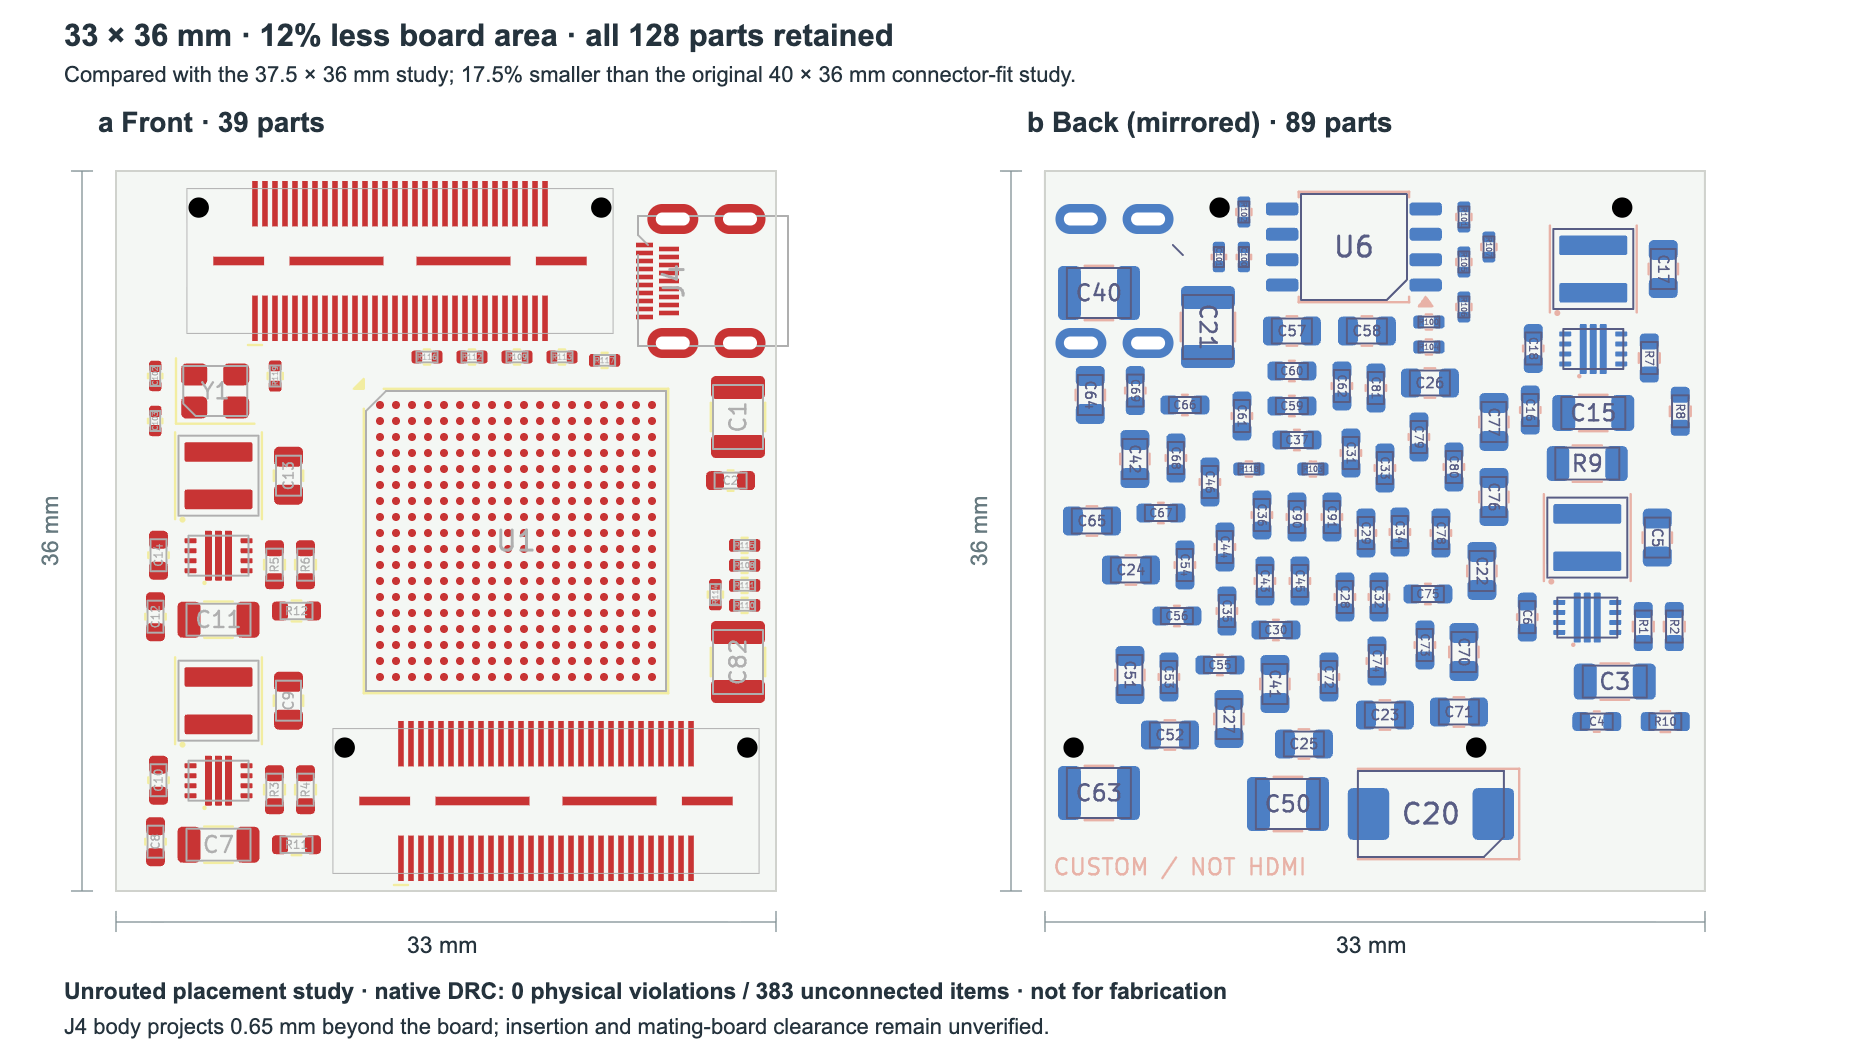
\includegraphics[width=\linewidth]{figures/Compact_Placement.png}}{\textbf{Native placement overview pending.}}

\textbf{Figure 1.} Native 33 $\times$ 36 mm placement, front and mirrored back. Only component geometry is shown; no connecting copper is present. The PCB rectangle is not the complete plug or mating-board envelope.

The reduction comes from repacking both faces and moving J5, J4, the back-side power groups, the clock group and selected support parts inward. U1 and J6 stay fixed. The existing converter groups retain their internal geometry. No decoupling capacitor, connector, flash, oscillator, strap or regulator was removed to obtain the smaller outline. There are no added debug headers, user LEDs or standalone test points in this candidate.

The front openings in the earlier core-only image are occupied by the two required mezzanine connectors in the complete placement study. The long back-side opening is mirrored relative to the front and can overlap a regulator or its required routing area on the opposite face. Empty drawing space therefore does not directly equal removable board area.

This is a demonstrated smaller placement, not proof of the smallest functional board. BGA escape, the power return paths, connector mating height, cable strain, protection components and thermal copper may require space that is currently blank. Assembly tolerances must be checked in addition to the saved CAD rules.
\textbf{Measured limits.} The smallest same-face courtyard-box gap is about 0.010 mm; the smallest fabrication-body-box gap is 0.360 mm. The nearest opposite-face courtyard-to-through-pad-box gap is 0.090 mm. The minimum copper-pad edge margin is 0.500 mm. These are native-geometry measurements, not approved assembly allowances.

J4's drawn body extends 0.65 mm beyond the PCB edge, giving a board-plus-drawn-body envelope of approximately \textbf{33.65 $\times$ 36 mm}; its courtyard extends 1.125 mm. The full mated assembly and plug envelope remain unverified. The earlier 37.5 mm and intermediate 34 mm candidates are preserved if routing or assembly needs more space.
\clearpage
\section{How the intended circuit works}
The following paths describe \emph{logical net assignments}. Every arrow still requires real copper in this placement. Parts and rails belong to the inherited 3.3 V boot/configuration version. The separate 1.8 V configuration / 2.5 V link-bank proposal is not integrated here.
\subsection{Power and sequencing}
J4.19 is assigned to \nolinkurl{LINK_12V}. It feeds the input capacitors and all four converters. This is a proposed custom power connection, not proof that an XEM8310 carrier or an ordinary micro-HDMI cable can safely supply it.

\begingroup\fontsize{9}{11.5}\selectfont\setlength{\tabcolsep}{2.8pt}\renewcommand{\arraystretch}{1.14}
\begin{longtable}{@{}P{23mm}P{86mm}P{59mm}@{}}
\toprule \textbf{Path} & \textbf{Assigned circuit} & \textbf{Why it exists} \\ \midrule
\endfirsthead\toprule \textbf{Path} & \textbf{Assigned circuit} & \textbf{Why it exists} \\ \midrule
\endhead\midrule\multicolumn{3}{r}{\small Continued on the next page}\endfoot\bottomrule\endlastfoot
Core & U2.2 $\rightarrow$ L1 $\rightarrow$ \nolinkurl{VCORE_REG_1V025} $\rightarrow$ R9 $\rightarrow$ \nolinkurl{VCCINT_1V0} & Powers FPGA logic and block RAM. R9 is a 15 milliohm series element. \\
Auxiliary & U3.2 $\rightarrow$ L2 $\rightarrow$ \nolinkurl{VCCAUX_1V8} & Powers FPGA auxiliary and analog supply domains. \\
Boot / config & U4.2 $\rightarrow$ L3 $\rightarrow$ \nolinkurl{VCC_CFG_3V3} & Supplies configuration I/O, flash, oscillator and pull-ups. \\
ASIC-facing I/O & U5.2 $\rightarrow$ L4 $\rightarrow$ \nolinkurl{VCC_ASIC_1V5} & Supplies selected FPGA I/O banks; external ASIC power delivery is not established. \\
Enable chain & \nolinkurl{LINK_12V} enables U2; \nolinkurl{PG_CORE} enables U3; \nolinkurl{PG_AUX} enables U4 and U5. & Power-good sequencing intent. Startup and discharge behaviour still require validation. \\
\end{longtable}\endgroup

The four TPS62135 converters use a local inductor, input and output capacitors, feedback divider and soft-start capacitor. Pin 11 is \textbf{VSEL}, tied to ground; it must not be mistaken for a second ground pin. Pin 3 is the ground pin. Pin 4 (FB2) is intentionally left open in this configuration. The pin roles were checked against TI's datasheet [1].

U2 senses the output \emph{before} R9. The nominal core voltage after R9 changes with current: a 1 A load produces about 15 mV drop and 15 mW dissipation in a 15 milliohm element. That arithmetic is not a load or thermal validation. FPGA activity, converter limits, capacitor bias loss and the actual supply tolerance still need analysis.

\subsection{Configuration, clock and programming}
U6 is the proposed 3.3 V configuration flash. U1.E9 drives its clock through R103; DQ0--DQ3 use R104--R107; U1.L13 controls chip select. The complete endpoint lists are in Appendices B--E. U6.7 is RESET/SIO3 for the stated Macronix part, not an assumed HOLD input [4].

R111--R113 encode M[2:0] = 001; R108--R110 pull up PROGRAM\_B, INIT\_B and DONE. R114 pulls PUDC\_B high. These inherited assignments document the master-SPI boot intent; compatible firmware, boot settings, reset recovery and a power-up test are not yet demonstrated [2].

Y1 provides a separate 32 MHz user clock. Y1.3 passes through R119 to U1.P17. Y1.1 is tied high to enable the oscillator; pins 2 and 4 are ground and supply [5]. JTAG uses J4.2/15/17/18 and dedicated FPGA pins, with R118 in the TDO path. J4.1 is a 3.3 V target-reference assignment, not an independently qualified power output.
\clearpage
\section{Pin budget, terminology and completeness}
The team correction is \textbf{117 ASIC-related signals}: 88 ASIC output/interface signals, 12 SPI data/control streams, nine shared controls, four board clocks and four additional SPI clocks. This is an interface budget, not a complete FPGA package pin count.

\begingroup\fontsize{9}{11.5}\selectfont\setlength{\tabcolsep}{2.8pt}\renewcommand{\arraystretch}{1.14}
\begin{longtable}{@{}P{53mm}P{17mm}P{98mm}@{}}
\toprule \textbf{Group} & \textbf{Count} & \textbf{Interpretation} \\ \midrule
\endfirsthead\toprule \textbf{Group} & \textbf{Count} & \textbf{Interpretation} \\ \midrule
\endhead\midrule\multicolumn{3}{r}{\small Continued on the next page}\endfoot\bottomrule\endlastfoot
ASIC output/interface & 88 & Eight groups of 11: 64 DATA1--8 lines plus eight each of CLK32MHz\_Out, READ and SYNC. \\
SPI data & 12 & Four stimulation SPI L, four stimulation SPI R, two non-stimulation SPI L and two non-stimulation SPI R. \\
Shared controls & 9 & \nolinkurl{CHIP_RESET, AC_IN, IMP_TST, FE_RESET, SPI_LATCH, STIM_CLK, STIM_START, STIM_EN, STIM_CHB} \\
Board clocks & 4 & One board clock per board in the supplied requirement. \\
SPI clocks & 4 & The four SPI\_CLK connections added in the team correction. \\
Total & 117 & Proposed across 120 mezzanine contacts, with three contacts spare. \\
\end{longtable}\endgroup

AC\_IN and IMP\_TST remain electrically unresolved: their names and tutorial diagrams alone do not establish safe direct FPGA voltage limits or whether conditioning is required. The full ASIC pad specification and timing contract are needed before allocating FPGA balls. The XEM8310 is an FPGA module used as the downstream endpoint; the required carrier, protocol, clocking and supply connection remain separate design work.

\textbf{Assigned} means that KiCad places endpoints on the same named logical net. \textbf{Unrouted} means no copper path has been built in this revision. \textbf{Unassigned} means no functional net has been allocated. \textbf{Intentional NC} marks a pin deliberately left open in the inherited core design; it is not a spare signal.

\begingroup\fontsize{9}{11.5}\selectfont\setlength{\tabcolsep}{2.8pt}\renewcommand{\arraystretch}{1.14}
\begin{longtable}{@{}P{53mm}P{17mm}P{98mm}@{}}
\toprule \textbf{Coverage} & \textbf{Count} & \textbf{Meaning} \\ \midrule
\endfirsthead\toprule \textbf{Coverage} & \textbf{Count} & \textbf{Meaning} \\ \midrule
\endhead\midrule\multicolumn{3}{r}{\small Continued on the next page}\endfoot\bottomrule\endlastfoot
Physical components & 128 & 82 capacitors, 32 resistors, four inductors, six ICs, three connectors and one oscillator. \\
Unique electrical endpoints & 758 & 421 assigned, 331 unassigned, six intentional NC. Every endpoint is listed in the appendices. \\
Numbered physical pads & 767 & Includes four shell pads sharing J4.SH, four ground lands sharing J5.G and four sharing J6.G. \\
Unnumbered records & 40 & 36 solder-paste-only apertures and four non-plated connector locating holes; these are not extra electrical pins. \\
All physical pad records & 807 & 767 numbered plus 40 unnumbered; preserved from the earlier placement. \\
Functional nets & 47 & KiCad placeholder unconnected names are excluded. The full peer list of each real net appears in Appendix E. \\
Unassigned breakdown & 331 & 203 FPGA user-I/O balls, eight reserved cable contacts, 120 mezzanine signal contacts. \\
Intentional NC & 6 & U1.L9 / L10 (DXN / DXP) and U2--U5 pin 4 (FB2). \\
\end{longtable}\endgroup

\clearpage\section{What must be resolved before release}
The 33 $\times$ 36 mm result improves placement. It does not close the earlier system uncertainties. The following issues directly affect whether this size can become a functioning board.

\begingroup\fontsize{9}{11.5}\selectfont\setlength{\tabcolsep}{2.8pt}\renewcommand{\arraystretch}{1.14}
\begin{longtable}{@{}P{50mm}P{122mm}@{}}
\toprule \textbf{Open item} & \textbf{Required next evidence / proposed owner} \\ \midrule
\endfirsthead\toprule \textbf{Open item} & \textbf{Required next evidence / proposed owner} \\ \midrule
\endhead\midrule\multicolumn{2}{r}{\small Continued on the next page}\endfoot\bottomrule\endlastfoot
ASIC electrical contract & ASIC design owner / Gerald: confirm all pad types, levels, drive strengths, reset states and setup/hold limits, especially AC\_IN and IMP\_TST. \\
FPGA assignment and bank rails & FPGA engineering: select all 117 FPGA balls and compatible banks/standards, then generate the schematic and XDC from one checked pin table. \\
Downstream link and power & FPGA + carrier engineering: define a realizable XEM8310 carrier connection, data protocol, clocking, cable pinout, current limit, length and protection. \\
One integrated circuit & PCB engineering: reconcile this 3.3 V core-derived layout with the separate rail revision, including C92/R122 and any selected replacement flash/oscillator. \\
Routing and stackup & PCB engineering + fabricator: route all power, ground, boot, clock, JTAG, ASIC and link nets; agree BGA escape rules, stackup and impedance. \\
Mechanical assembly & PCB engineering + assembler: approve the connector body overhang, mating-board offsets, height, retention, courtyard tolerances and dual-side assembly access. \\
Part values and procurement & PCB engineering: finish all TBD order codes, check footprint/part matches and qualify capacitor effective values and the required decoupling count. \\
Measured acceptance & FPGA + lab team: cold boot, brownout/recovery, all-channel capture, sustained transfer, error rate, power and thermal tests on actual hardware. \\
\end{longtable}\endgroup

The current complete-board design has no manufacturing release. A DRC pass does not demonstrate signal integrity, power integrity, thermal margin, assembler acceptance or working firmware. It also does not check the 117 signals that have no assigned PCB net yet.

\textbf{Further reduction path.} The next useful size decision is an integrated routing trial with the required protection and bank-voltage choices. A changed connector orientation or a smaller power architecture may reduce size further, but cannot be approved by deleting components or trimming blank drawing space alone.
\clearpage\appendix
\section{Every component: purpose and connections}
All 128 physical components appear below. Values and order codes describe the saved candidate; TBD is preserved wherever selection is incomplete. The table is a design ledger, not an approved purchase BOM. For two-terminal components, both pins are listed here. Larger devices refer to their complete pin tables later in this report.

\begingroup\fontsize{9}{11.5}\selectfont\setlength{\tabcolsep}{2.8pt}\renewcommand{\arraystretch}{1.14}
\begin{longtable}{@{}P{27mm}P{84mm}P{57mm}@{}}
\toprule \textbf{Ref. / value / face} & \textbf{Why it is here / saved order code} & \textbf{Actual pin-to-net assignment} \\ \midrule
\endfirsthead\toprule \textbf{Ref. / value / face} & \textbf{Why it is here / saved order code} & \textbf{Actual pin-to-net assignment} \\ \midrule
\endhead\midrule\multicolumn{3}{r}{\small Continued on the next page}\endfoot\bottomrule\endlastfoot
\textbf{C1}\newline 47u 25V X5R\newline {\color{muted}Front} & Cable-input bulk charge reservoir between LINK\_12V and ground. Does not replace input protection.\newline {\color{muted}Order: \nolinkurl{MSAST32MAB5476MPNDT1}} & \nolinkurl{1}: \nolinkurl{LINK_12V}\newline \nolinkurl{2}: \nolinkurl{GND} \\
\textbf{C2}\newline 100n 100V X7R\newline {\color{muted}Front} & Cable-input local high-frequency bypass between LINK\_12V and ground. Does not replace input protection.\newline {\color{muted}Order: \nolinkurl{GRM188R72A104KA35D}} & \nolinkurl{1}: \nolinkurl{LINK_12V}\newline \nolinkurl{2}: \nolinkurl{GND} \\
\textbf{C3}\newline 22u 25V X5R\newline {\color{muted}Back} & Local converter input reservoir on LINK\_12V. Nominal 22 uF / 25 V; effective capacitance at bias and placement need qualification.\newline {\color{muted}Order: \nolinkurl{MSAST31LBB5226MTNA01}} & \nolinkurl{1}: \nolinkurl{LINK_12V}\newline \nolinkurl{2}: \nolinkurl{GND} \\
\textbf{C4}\newline 100n 100V X7R\newline {\color{muted}Back} & Small local converter input bypass from LINK\_12V to ground.\newline {\color{muted}Order: \nolinkurl{GRM188R72A104KA35D}} & \nolinkurl{1}: \nolinkurl{LINK_12V}\newline \nolinkurl{2}: \nolinkurl{GND} \\
\textbf{C5}\newline 22u 16V X5R\newline {\color{muted}Back} & Local converter output capacitor and voltage-sense node; keep close to inductor/ground return.\newline {\color{muted}Order: \nolinkurl{EMK212BBJ226MG-T}} & \nolinkurl{1}: \nolinkurl{VCORE_REG_1V025}\newline \nolinkurl{2}: \nolinkurl{GND} \\
\textbf{C6}\newline 10n 50V X7R\newline {\color{muted}Back} & Soft-start capacitor from SS\_CORE to ground; sets the converter reference ramp.\newline {\color{muted}Order: TBD - manufacturer/order code not selected} & \nolinkurl{1}: \nolinkurl{SS_CORE}\newline \nolinkurl{2}: \nolinkurl{GND} \\
\textbf{C7}\newline 22u 25V X5R\newline {\color{muted}Front} & Local converter input reservoir on LINK\_12V. Nominal 22 uF / 25 V; effective capacitance at bias and placement need qualification.\newline {\color{muted}Order: \nolinkurl{MSAST31LBB5226MTNA01}} & \nolinkurl{1}: \nolinkurl{LINK_12V}\newline \nolinkurl{2}: \nolinkurl{GND} \\
\textbf{C8}\newline 100n 100V X7R\newline {\color{muted}Front} & Small local converter input bypass from LINK\_12V to ground.\newline {\color{muted}Order: \nolinkurl{GRM188R72A104KA35D}} & \nolinkurl{1}: \nolinkurl{LINK_12V}\newline \nolinkurl{2}: \nolinkurl{GND} \\
\textbf{C9}\newline 22u 16V X5R\newline {\color{muted}Front} & Local converter output capacitor and voltage-sense node; keep close to inductor/ground return.\newline {\color{muted}Order: \nolinkurl{EMK212BBJ226MG-T}} & \nolinkurl{1}: \nolinkurl{VCCAUX_1V8}\newline \nolinkurl{2}: \nolinkurl{GND} \\
\textbf{C10}\newline 10n 50V X7R\newline {\color{muted}Front} & Soft-start capacitor from SS\_AUX to ground; sets the converter reference ramp.\newline {\color{muted}Order: TBD - manufacturer/order code not selected} & \nolinkurl{1}: \nolinkurl{SS_AUX}\newline \nolinkurl{2}: \nolinkurl{GND} \\
\textbf{C11}\newline 22u 25V X5R\newline {\color{muted}Front} & Local converter input reservoir on LINK\_12V. Nominal 22 uF / 25 V; effective capacitance at bias and placement need qualification.\newline {\color{muted}Order: \nolinkurl{MSAST31LBB5226MTNA01}} & \nolinkurl{1}: \nolinkurl{LINK_12V}\newline \nolinkurl{2}: \nolinkurl{GND} \\
\textbf{C12}\newline 100n 100V X7R\newline {\color{muted}Front} & Small local converter input bypass from LINK\_12V to ground.\newline {\color{muted}Order: \nolinkurl{GRM188R72A104KA35D}} & \nolinkurl{1}: \nolinkurl{LINK_12V}\newline \nolinkurl{2}: \nolinkurl{GND} \\
\textbf{C13}\newline 22u 16V X5R\newline {\color{muted}Front} & Local converter output capacitor and voltage-sense node; keep close to inductor/ground return.\newline {\color{muted}Order: \nolinkurl{EMK212BBJ226MG-T}} & \nolinkurl{1}: \nolinkurl{VCC_CFG_3V3}\newline \nolinkurl{2}: \nolinkurl{GND} \\
\textbf{C14}\newline 10n 50V X7R\newline {\color{muted}Front} & Soft-start capacitor from SS\_CFG to ground; sets the converter reference ramp.\newline {\color{muted}Order: TBD - manufacturer/order code not selected} & \nolinkurl{1}: \nolinkurl{SS_CFG}\newline \nolinkurl{2}: \nolinkurl{GND} \\
\textbf{C15}\newline 22u 25V X5R\newline {\color{muted}Back} & Local converter input reservoir on LINK\_12V. Nominal 22 uF / 25 V; effective capacitance at bias and placement need qualification.\newline {\color{muted}Order: \nolinkurl{MSAST31LBB5226MTNA01}} & \nolinkurl{1}: \nolinkurl{LINK_12V}\newline \nolinkurl{2}: \nolinkurl{GND} \\
\textbf{C16}\newline 100n 100V X7R\newline {\color{muted}Back} & Small local converter input bypass from LINK\_12V to ground.\newline {\color{muted}Order: \nolinkurl{GRM188R72A104KA35D}} & \nolinkurl{1}: \nolinkurl{LINK_12V}\newline \nolinkurl{2}: \nolinkurl{GND} \\
\textbf{C17}\newline 22u 16V X5R\newline {\color{muted}Back} & Local converter output capacitor and voltage-sense node; keep close to inductor/ground return.\newline {\color{muted}Order: \nolinkurl{EMK212BBJ226MG-T}} & \nolinkurl{1}: \nolinkurl{VCC_ASIC_1V5}\newline \nolinkurl{2}: \nolinkurl{GND} \\
\textbf{C18}\newline 10n 50V X7R\newline {\color{muted}Back} & Soft-start capacitor from SS\_ASIC to ground; sets the converter reference ramp.\newline {\color{muted}Order: TBD - manufacturer/order code not selected} & \nolinkurl{1}: \nolinkurl{SS_ASIC}\newline \nolinkurl{2}: \nolinkurl{GND} \\
\textbf{C20}\newline 330u 2.5V polymer ESR25m\newline {\color{muted}Back} & Distributed logic-core decoupling on VCCINT\_1V0. This inherited value/count is a design candidate, not a demonstrated minimum.\newline {\color{muted}Order: \nolinkurl{T520V337M2R5ATE025}} & \nolinkurl{1}: \nolinkurl{VCCINT_1V0}\newline \nolinkurl{2}: \nolinkurl{GND} \\
\textbf{C21}\newline 100u 6.3V X5R\newline {\color{muted}Back} & Distributed block-RAM decoupling on VCCINT\_1V0. This inherited value/count is a design candidate, not a demonstrated minimum.\newline {\color{muted}Order: \nolinkurl{GRM32ER60J107ME20L}} & \nolinkurl{1}: \nolinkurl{VCCINT_1V0}\newline \nolinkurl{2}: \nolinkurl{GND} \\
\textbf{C22}\newline 4.7u 10V X7R\newline {\color{muted}Back} & Distributed logic-core decoupling on VCCINT\_1V0. This inherited value/count is a design candidate, not a demonstrated minimum.\newline {\color{muted}Order: \nolinkurl{GRM21BR71A475KA73L}} & \nolinkurl{1}: \nolinkurl{VCCINT_1V0}\newline \nolinkurl{2}: \nolinkurl{GND} \\
\textbf{C23}\newline 4.7u 10V X7R\newline {\color{muted}Back} & Distributed logic-core decoupling on VCCINT\_1V0. This inherited value/count is a design candidate, not a demonstrated minimum.\newline {\color{muted}Order: \nolinkurl{GRM21BR71A475KA73L}} & \nolinkurl{1}: \nolinkurl{VCCINT_1V0}\newline \nolinkurl{2}: \nolinkurl{GND} \\
\textbf{C24}\newline 4.7u 10V X7R\newline {\color{muted}Back} & Distributed logic-core decoupling on VCCINT\_1V0. This inherited value/count is a design candidate, not a demonstrated minimum.\newline {\color{muted}Order: \nolinkurl{GRM21BR71A475KA73L}} & \nolinkurl{1}: \nolinkurl{VCCINT_1V0}\newline \nolinkurl{2}: \nolinkurl{GND} \\
\textbf{C25}\newline 4.7u 10V X7R\newline {\color{muted}Back} & Distributed logic-core decoupling on VCCINT\_1V0. This inherited value/count is a design candidate, not a demonstrated minimum.\newline {\color{muted}Order: \nolinkurl{GRM21BR71A475KA73L}} & \nolinkurl{1}: \nolinkurl{VCCINT_1V0}\newline \nolinkurl{2}: \nolinkurl{GND} \\
\textbf{C26}\newline 4.7u 10V X7R\newline {\color{muted}Back} & Distributed logic-core decoupling on VCCINT\_1V0. This inherited value/count is a design candidate, not a demonstrated minimum.\newline {\color{muted}Order: \nolinkurl{GRM21BR71A475KA73L}} & \nolinkurl{1}: \nolinkurl{VCCINT_1V0}\newline \nolinkurl{2}: \nolinkurl{GND} \\
\textbf{C27}\newline 4.7u 10V X7R\newline {\color{muted}Back} & Distributed logic-core decoupling on VCCINT\_1V0. This inherited value/count is a design candidate, not a demonstrated minimum.\newline {\color{muted}Order: \nolinkurl{GRM21BR71A475KA73L}} & \nolinkurl{1}: \nolinkurl{VCCINT_1V0}\newline \nolinkurl{2}: \nolinkurl{GND} \\
\textbf{C28}\newline 470n 6.3V X7R\newline {\color{muted}Back} & Distributed logic-core decoupling on VCCINT\_1V0. This inherited value/count is a design candidate, not a demonstrated minimum.\newline {\color{muted}Order: \nolinkurl{GRM188R70J474KA01D}} & \nolinkurl{1}: \nolinkurl{VCCINT_1V0}\newline \nolinkurl{2}: \nolinkurl{GND} \\
\textbf{C29}\newline 470n 6.3V X7R\newline {\color{muted}Back} & Distributed logic-core decoupling on VCCINT\_1V0. This inherited value/count is a design candidate, not a demonstrated minimum.\newline {\color{muted}Order: \nolinkurl{GRM188R70J474KA01D}} & \nolinkurl{1}: \nolinkurl{VCCINT_1V0}\newline \nolinkurl{2}: \nolinkurl{GND} \\
\textbf{C30}\newline 470n 6.3V X7R\newline {\color{muted}Back} & Distributed logic-core decoupling on VCCINT\_1V0. This inherited value/count is a design candidate, not a demonstrated minimum.\newline {\color{muted}Order: \nolinkurl{GRM188R70J474KA01D}} & \nolinkurl{1}: \nolinkurl{VCCINT_1V0}\newline \nolinkurl{2}: \nolinkurl{GND} \\
\textbf{C31}\newline 470n 6.3V X7R\newline {\color{muted}Back} & Distributed logic-core decoupling on VCCINT\_1V0. This inherited value/count is a design candidate, not a demonstrated minimum.\newline {\color{muted}Order: \nolinkurl{GRM188R70J474KA01D}} & \nolinkurl{1}: \nolinkurl{VCCINT_1V0}\newline \nolinkurl{2}: \nolinkurl{GND} \\
\textbf{C32}\newline 470n 6.3V X7R\newline {\color{muted}Back} & Distributed logic-core decoupling on VCCINT\_1V0. This inherited value/count is a design candidate, not a demonstrated minimum.\newline {\color{muted}Order: \nolinkurl{GRM188R70J474KA01D}} & \nolinkurl{1}: \nolinkurl{VCCINT_1V0}\newline \nolinkurl{2}: \nolinkurl{GND} \\
\textbf{C33}\newline 470n 6.3V X7R\newline {\color{muted}Back} & Distributed logic-core decoupling on VCCINT\_1V0. This inherited value/count is a design candidate, not a demonstrated minimum.\newline {\color{muted}Order: \nolinkurl{GRM188R70J474KA01D}} & \nolinkurl{1}: \nolinkurl{VCCINT_1V0}\newline \nolinkurl{2}: \nolinkurl{GND} \\
\textbf{C34}\newline 470n 6.3V X7R\newline {\color{muted}Back} & Distributed logic-core decoupling on VCCINT\_1V0. This inherited value/count is a design candidate, not a demonstrated minimum.\newline {\color{muted}Order: \nolinkurl{GRM188R70J474KA01D}} & \nolinkurl{1}: \nolinkurl{VCCINT_1V0}\newline \nolinkurl{2}: \nolinkurl{GND} \\
\textbf{C35}\newline 470n 6.3V X7R\newline {\color{muted}Back} & Distributed logic-core decoupling on VCCINT\_1V0. This inherited value/count is a design candidate, not a demonstrated minimum.\newline {\color{muted}Order: \nolinkurl{GRM188R70J474KA01D}} & \nolinkurl{1}: \nolinkurl{VCCINT_1V0}\newline \nolinkurl{2}: \nolinkurl{GND} \\
\textbf{C36}\newline 470n 6.3V X7R\newline {\color{muted}Back} & Distributed block-RAM decoupling on VCCINT\_1V0. This inherited value/count is a design candidate, not a demonstrated minimum.\newline {\color{muted}Order: \nolinkurl{GRM188R70J474KA01D}} & \nolinkurl{1}: \nolinkurl{VCCINT_1V0}\newline \nolinkurl{2}: \nolinkurl{GND} \\
\textbf{C37}\newline 470n 6.3V X7R\newline {\color{muted}Back} & Distributed block-RAM decoupling on VCCINT\_1V0. This inherited value/count is a design candidate, not a demonstrated minimum.\newline {\color{muted}Order: \nolinkurl{GRM188R70J474KA01D}} & \nolinkurl{1}: \nolinkurl{VCCINT_1V0}\newline \nolinkurl{2}: \nolinkurl{GND} \\
\textbf{C40}\newline 47u 6.3V X7R\newline {\color{muted}Back} & Distributed auxiliary decoupling on VCCAUX\_1V8. This inherited value/count is a design candidate, not a demonstrated minimum.\newline {\color{muted}Order: \nolinkurl{GRM32ER70J476ME20L}} & \nolinkurl{1}: \nolinkurl{VCCAUX_1V8}\newline \nolinkurl{2}: \nolinkurl{GND} \\
\textbf{C41}\newline 4.7u 10V X7R\newline {\color{muted}Back} & Distributed auxiliary decoupling on VCCAUX\_1V8. This inherited value/count is a design candidate, not a demonstrated minimum.\newline {\color{muted}Order: \nolinkurl{GRM21BR71A475KA73L}} & \nolinkurl{1}: \nolinkurl{VCCAUX_1V8}\newline \nolinkurl{2}: \nolinkurl{GND} \\
\textbf{C42}\newline 4.7u 10V X7R\newline {\color{muted}Back} & Distributed auxiliary decoupling on VCCAUX\_1V8. This inherited value/count is a design candidate, not a demonstrated minimum.\newline {\color{muted}Order: \nolinkurl{GRM21BR71A475KA73L}} & \nolinkurl{1}: \nolinkurl{VCCAUX_1V8}\newline \nolinkurl{2}: \nolinkurl{GND} \\
\textbf{C43}\newline 470n 6.3V X7R\newline {\color{muted}Back} & Distributed auxiliary decoupling on VCCAUX\_1V8. This inherited value/count is a design candidate, not a demonstrated minimum.\newline {\color{muted}Order: \nolinkurl{GRM188R70J474KA01D}} & \nolinkurl{1}: \nolinkurl{VCCAUX_1V8}\newline \nolinkurl{2}: \nolinkurl{GND} \\
\textbf{C44}\newline 470n 6.3V X7R\newline {\color{muted}Back} & Distributed auxiliary decoupling on VCCAUX\_1V8. This inherited value/count is a design candidate, not a demonstrated minimum.\newline {\color{muted}Order: \nolinkurl{GRM188R70J474KA01D}} & \nolinkurl{1}: \nolinkurl{VCCAUX_1V8}\newline \nolinkurl{2}: \nolinkurl{GND} \\
\textbf{C45}\newline 470n 6.3V X7R\newline {\color{muted}Back} & Distributed auxiliary decoupling on VCCAUX\_1V8. This inherited value/count is a design candidate, not a demonstrated minimum.\newline {\color{muted}Order: \nolinkurl{GRM188R70J474KA01D}} & \nolinkurl{1}: \nolinkurl{VCCAUX_1V8}\newline \nolinkurl{2}: \nolinkurl{GND} \\
\textbf{C46}\newline 470n 6.3V X7R\newline {\color{muted}Back} & Distributed auxiliary decoupling on VCCAUX\_1V8. This inherited value/count is a design candidate, not a demonstrated minimum.\newline {\color{muted}Order: \nolinkurl{GRM188R70J474KA01D}} & \nolinkurl{1}: \nolinkurl{VCCAUX_1V8}\newline \nolinkurl{2}: \nolinkurl{GND} \\
\textbf{C50}\newline 47u 6.3V X7R\newline {\color{muted}Back} & Distributed configuration-bank decoupling on VCC\_CFG\_3V3. This inherited value/count is a design candidate, not a demonstrated minimum.\newline {\color{muted}Order: \nolinkurl{GRM32ER70J476ME20L}} & \nolinkurl{1}: \nolinkurl{VCC_CFG_3V3}\newline \nolinkurl{2}: \nolinkurl{GND} \\
\textbf{C51}\newline 4.7u 10V X7R\newline {\color{muted}Back} & Distributed I/O bank 14 decoupling on VCC\_CFG\_3V3. This inherited value/count is a design candidate, not a demonstrated minimum.\newline {\color{muted}Order: \nolinkurl{GRM21BR71A475KA73L}} & \nolinkurl{1}: \nolinkurl{VCC_CFG_3V3}\newline \nolinkurl{2}: \nolinkurl{GND} \\
\textbf{C52}\newline 4.7u 10V X7R\newline {\color{muted}Back} & Distributed I/O bank 14 decoupling on VCC\_CFG\_3V3. This inherited value/count is a design candidate, not a demonstrated minimum.\newline {\color{muted}Order: \nolinkurl{GRM21BR71A475KA73L}} & \nolinkurl{1}: \nolinkurl{VCC_CFG_3V3}\newline \nolinkurl{2}: \nolinkurl{GND} \\
\textbf{C53}\newline 470n 6.3V X7R\newline {\color{muted}Back} & Distributed I/O bank 14 decoupling on VCC\_CFG\_3V3. This inherited value/count is a design candidate, not a demonstrated minimum.\newline {\color{muted}Order: \nolinkurl{GRM188R70J474KA01D}} & \nolinkurl{1}: \nolinkurl{VCC_CFG_3V3}\newline \nolinkurl{2}: \nolinkurl{GND} \\
\textbf{C54}\newline 470n 6.3V X7R\newline {\color{muted}Back} & Distributed I/O bank 14 decoupling on VCC\_CFG\_3V3. This inherited value/count is a design candidate, not a demonstrated minimum.\newline {\color{muted}Order: \nolinkurl{GRM188R70J474KA01D}} & \nolinkurl{1}: \nolinkurl{VCC_CFG_3V3}\newline \nolinkurl{2}: \nolinkurl{GND} \\
\textbf{C55}\newline 470n 6.3V X7R\newline {\color{muted}Back} & Distributed I/O bank 14 decoupling on VCC\_CFG\_3V3. This inherited value/count is a design candidate, not a demonstrated minimum.\newline {\color{muted}Order: \nolinkurl{GRM188R70J474KA01D}} & \nolinkurl{1}: \nolinkurl{VCC_CFG_3V3}\newline \nolinkurl{2}: \nolinkurl{GND} \\
\textbf{C56}\newline 470n 6.3V X7R\newline {\color{muted}Back} & Distributed I/O bank 14 decoupling on VCC\_CFG\_3V3. This inherited value/count is a design candidate, not a demonstrated minimum.\newline {\color{muted}Order: \nolinkurl{GRM188R70J474KA01D}} & \nolinkurl{1}: \nolinkurl{VCC_CFG_3V3}\newline \nolinkurl{2}: \nolinkurl{GND} \\
\textbf{C57}\newline 4.7u 10V X7R\newline {\color{muted}Back} & Distributed I/O bank 16 decoupling on VCC\_CFG\_3V3. This inherited value/count is a design candidate, not a demonstrated minimum.\newline {\color{muted}Order: \nolinkurl{GRM21BR71A475KA73L}} & \nolinkurl{1}: \nolinkurl{VCC_CFG_3V3}\newline \nolinkurl{2}: \nolinkurl{GND} \\
\textbf{C58}\newline 4.7u 10V X7R\newline {\color{muted}Back} & Distributed I/O bank 16 decoupling on VCC\_CFG\_3V3. This inherited value/count is a design candidate, not a demonstrated minimum.\newline {\color{muted}Order: \nolinkurl{GRM21BR71A475KA73L}} & \nolinkurl{1}: \nolinkurl{VCC_CFG_3V3}\newline \nolinkurl{2}: \nolinkurl{GND} \\
\textbf{C59}\newline 470n 6.3V X7R\newline {\color{muted}Back} & Distributed I/O bank 16 decoupling on VCC\_CFG\_3V3. This inherited value/count is a design candidate, not a demonstrated minimum.\newline {\color{muted}Order: \nolinkurl{GRM188R70J474KA01D}} & \nolinkurl{1}: \nolinkurl{VCC_CFG_3V3}\newline \nolinkurl{2}: \nolinkurl{GND} \\
\textbf{C60}\newline 470n 6.3V X7R\newline {\color{muted}Back} & Distributed I/O bank 16 decoupling on VCC\_CFG\_3V3. This inherited value/count is a design candidate, not a demonstrated minimum.\newline {\color{muted}Order: \nolinkurl{GRM188R70J474KA01D}} & \nolinkurl{1}: \nolinkurl{VCC_CFG_3V3}\newline \nolinkurl{2}: \nolinkurl{GND} \\
\textbf{C61}\newline 470n 6.3V X7R\newline {\color{muted}Back} & Distributed I/O bank 16 decoupling on VCC\_CFG\_3V3. This inherited value/count is a design candidate, not a demonstrated minimum.\newline {\color{muted}Order: \nolinkurl{GRM188R70J474KA01D}} & \nolinkurl{1}: \nolinkurl{VCC_CFG_3V3}\newline \nolinkurl{2}: \nolinkurl{GND} \\
\textbf{C62}\newline 470n 6.3V X7R\newline {\color{muted}Back} & Distributed I/O bank 16 decoupling on VCC\_CFG\_3V3. This inherited value/count is a design candidate, not a demonstrated minimum.\newline {\color{muted}Order: \nolinkurl{GRM188R70J474KA01D}} & \nolinkurl{1}: \nolinkurl{VCC_CFG_3V3}\newline \nolinkurl{2}: \nolinkurl{GND} \\
\textbf{C63}\newline 47u 6.3V X7R\newline {\color{muted}Back} & Distributed configuration / I/O bulk decoupling on VCC\_CFG\_3V3. This inherited value/count is a design candidate, not a demonstrated minimum.\newline {\color{muted}Order: \nolinkurl{GRM32ER70J476ME20L}} & \nolinkurl{1}: \nolinkurl{VCC_CFG_3V3}\newline \nolinkurl{2}: \nolinkurl{GND} \\
\textbf{C64}\newline 4.7u 10V X7R\newline {\color{muted}Back} & Distributed I/O bank 15 decoupling on VCC\_ASIC\_1V5. This inherited value/count is a design candidate, not a demonstrated minimum.\newline {\color{muted}Order: \nolinkurl{GRM21BR71A475KA73L}} & \nolinkurl{1}: \nolinkurl{VCC_ASIC_1V5}\newline \nolinkurl{2}: \nolinkurl{GND} \\
\textbf{C65}\newline 4.7u 10V X7R\newline {\color{muted}Back} & Distributed I/O bank 15 decoupling on VCC\_ASIC\_1V5. This inherited value/count is a design candidate, not a demonstrated minimum.\newline {\color{muted}Order: \nolinkurl{GRM21BR71A475KA73L}} & \nolinkurl{1}: \nolinkurl{VCC_ASIC_1V5}\newline \nolinkurl{2}: \nolinkurl{GND} \\
\textbf{C66}\newline 470n 6.3V X7R\newline {\color{muted}Back} & Distributed I/O bank 15 decoupling on VCC\_ASIC\_1V5. This inherited value/count is a design candidate, not a demonstrated minimum.\newline {\color{muted}Order: \nolinkurl{GRM188R70J474KA01D}} & \nolinkurl{1}: \nolinkurl{VCC_ASIC_1V5}\newline \nolinkurl{2}: \nolinkurl{GND} \\
\textbf{C67}\newline 470n 6.3V X7R\newline {\color{muted}Back} & Distributed I/O bank 15 decoupling on VCC\_ASIC\_1V5. This inherited value/count is a design candidate, not a demonstrated minimum.\newline {\color{muted}Order: \nolinkurl{GRM188R70J474KA01D}} & \nolinkurl{1}: \nolinkurl{VCC_ASIC_1V5}\newline \nolinkurl{2}: \nolinkurl{GND} \\
\textbf{C68}\newline 470n 6.3V X7R\newline {\color{muted}Back} & Distributed I/O bank 15 decoupling on VCC\_ASIC\_1V5. This inherited value/count is a design candidate, not a demonstrated minimum.\newline {\color{muted}Order: \nolinkurl{GRM188R70J474KA01D}} & \nolinkurl{1}: \nolinkurl{VCC_ASIC_1V5}\newline \nolinkurl{2}: \nolinkurl{GND} \\
\textbf{C69}\newline 470n 6.3V X7R\newline {\color{muted}Back} & Distributed I/O bank 15 decoupling on VCC\_ASIC\_1V5. This inherited value/count is a design candidate, not a demonstrated minimum.\newline {\color{muted}Order: \nolinkurl{GRM188R70J474KA01D}} & \nolinkurl{1}: \nolinkurl{VCC_ASIC_1V5}\newline \nolinkurl{2}: \nolinkurl{GND} \\
\textbf{C70}\newline 4.7u 10V X7R\newline {\color{muted}Back} & Distributed I/O bank 34 decoupling on VCC\_ASIC\_1V5. This inherited value/count is a design candidate, not a demonstrated minimum.\newline {\color{muted}Order: \nolinkurl{GRM21BR71A475KA73L}} & \nolinkurl{1}: \nolinkurl{VCC_ASIC_1V5}\newline \nolinkurl{2}: \nolinkurl{GND} \\
\textbf{C71}\newline 4.7u 10V X7R\newline {\color{muted}Back} & Distributed I/O bank 34 decoupling on VCC\_ASIC\_1V5. This inherited value/count is a design candidate, not a demonstrated minimum.\newline {\color{muted}Order: \nolinkurl{GRM21BR71A475KA73L}} & \nolinkurl{1}: \nolinkurl{VCC_ASIC_1V5}\newline \nolinkurl{2}: \nolinkurl{GND} \\
\textbf{C72}\newline 470n 6.3V X7R\newline {\color{muted}Back} & Distributed I/O bank 34 decoupling on VCC\_ASIC\_1V5. This inherited value/count is a design candidate, not a demonstrated minimum.\newline {\color{muted}Order: \nolinkurl{GRM188R70J474KA01D}} & \nolinkurl{1}: \nolinkurl{VCC_ASIC_1V5}\newline \nolinkurl{2}: \nolinkurl{GND} \\
\textbf{C73}\newline 470n 6.3V X7R\newline {\color{muted}Back} & Distributed I/O bank 34 decoupling on VCC\_ASIC\_1V5. This inherited value/count is a design candidate, not a demonstrated minimum.\newline {\color{muted}Order: \nolinkurl{GRM188R70J474KA01D}} & \nolinkurl{1}: \nolinkurl{VCC_ASIC_1V5}\newline \nolinkurl{2}: \nolinkurl{GND} \\
\textbf{C74}\newline 470n 6.3V X7R\newline {\color{muted}Back} & Distributed I/O bank 34 decoupling on VCC\_ASIC\_1V5. This inherited value/count is a design candidate, not a demonstrated minimum.\newline {\color{muted}Order: \nolinkurl{GRM188R70J474KA01D}} & \nolinkurl{1}: \nolinkurl{VCC_ASIC_1V5}\newline \nolinkurl{2}: \nolinkurl{GND} \\
\textbf{C75}\newline 470n 6.3V X7R\newline {\color{muted}Back} & Distributed I/O bank 34 decoupling on VCC\_ASIC\_1V5. This inherited value/count is a design candidate, not a demonstrated minimum.\newline {\color{muted}Order: \nolinkurl{GRM188R70J474KA01D}} & \nolinkurl{1}: \nolinkurl{VCC_ASIC_1V5}\newline \nolinkurl{2}: \nolinkurl{GND} \\
\textbf{C76}\newline 4.7u 10V X7R\newline {\color{muted}Back} & Distributed I/O bank 35 decoupling on VCC\_ASIC\_1V5. This inherited value/count is a design candidate, not a demonstrated minimum.\newline {\color{muted}Order: \nolinkurl{GRM21BR71A475KA73L}} & \nolinkurl{1}: \nolinkurl{VCC_ASIC_1V5}\newline \nolinkurl{2}: \nolinkurl{GND} \\
\textbf{C77}\newline 4.7u 10V X7R\newline {\color{muted}Back} & Distributed I/O bank 35 decoupling on VCC\_ASIC\_1V5. This inherited value/count is a design candidate, not a demonstrated minimum.\newline {\color{muted}Order: \nolinkurl{GRM21BR71A475KA73L}} & \nolinkurl{1}: \nolinkurl{VCC_ASIC_1V5}\newline \nolinkurl{2}: \nolinkurl{GND} \\
\textbf{C78}\newline 470n 6.3V X7R\newline {\color{muted}Back} & Distributed I/O bank 35 decoupling on VCC\_ASIC\_1V5. This inherited value/count is a design candidate, not a demonstrated minimum.\newline {\color{muted}Order: \nolinkurl{GRM188R70J474KA01D}} & \nolinkurl{1}: \nolinkurl{VCC_ASIC_1V5}\newline \nolinkurl{2}: \nolinkurl{GND} \\
\textbf{C79}\newline 470n 6.3V X7R\newline {\color{muted}Back} & Distributed I/O bank 35 decoupling on VCC\_ASIC\_1V5. This inherited value/count is a design candidate, not a demonstrated minimum.\newline {\color{muted}Order: \nolinkurl{GRM188R70J474KA01D}} & \nolinkurl{1}: \nolinkurl{VCC_ASIC_1V5}\newline \nolinkurl{2}: \nolinkurl{GND} \\
\textbf{C80}\newline 470n 6.3V X7R\newline {\color{muted}Back} & Distributed I/O bank 35 decoupling on VCC\_ASIC\_1V5. This inherited value/count is a design candidate, not a demonstrated minimum.\newline {\color{muted}Order: \nolinkurl{GRM188R70J474KA01D}} & \nolinkurl{1}: \nolinkurl{VCC_ASIC_1V5}\newline \nolinkurl{2}: \nolinkurl{GND} \\
\textbf{C81}\newline 470n 6.3V X7R\newline {\color{muted}Back} & Distributed I/O bank 35 decoupling on VCC\_ASIC\_1V5. This inherited value/count is a design candidate, not a demonstrated minimum.\newline {\color{muted}Order: \nolinkurl{GRM188R70J474KA01D}} & \nolinkurl{1}: \nolinkurl{VCC_ASIC_1V5}\newline \nolinkurl{2}: \nolinkurl{GND} \\
\textbf{C82}\newline 47u 6.3V X7R\newline {\color{muted}Front} & Distributed ASIC-facing I/O bulk decoupling on VCC\_ASIC\_1V5. This inherited value/count is a design candidate, not a demonstrated minimum.\newline {\color{muted}Order: \nolinkurl{GRM32ER70J476ME20L}} & \nolinkurl{1}: \nolinkurl{VCC_ASIC_1V5}\newline \nolinkurl{2}: \nolinkurl{GND} \\
\textbf{C90}\newline 100n 16V X7R\newline {\color{muted}Back} & Bypass for the FPGA analog/XADC supply domain, tied to the auxiliary rail in this design.\newline {\color{muted}Order: TBD - manufacturer/order code not selected} & \nolinkurl{1}: \nolinkurl{VCCAUX_1V8}\newline \nolinkurl{2}: \nolinkurl{GND} \\
\textbf{C91}\newline 1u 10V X7R\newline {\color{muted}Back} & Bypass for the FPGA analog/XADC supply domain, tied to the auxiliary rail in this design.\newline {\color{muted}Order: TBD - manufacturer/order code not selected} & \nolinkurl{1}: \nolinkurl{VCCAUX_1V8}\newline \nolinkurl{2}: \nolinkurl{GND} \\
\textbf{C100}\newline 100n\newline {\color{muted}Back} & Local flash supply decoupling from 3.3 V to ground.\newline {\color{muted}Order: TBD - manufacturer/order code not selected} & \nolinkurl{1}: \nolinkurl{VCC_CFG_3V3}\newline \nolinkurl{2}: \nolinkurl{GND} \\
\textbf{C101}\newline 1u\newline {\color{muted}Back} & Local flash supply decoupling from 3.3 V to ground.\newline {\color{muted}Order: TBD - manufacturer/order code not selected} & \nolinkurl{1}: \nolinkurl{VCC_CFG_3V3}\newline \nolinkurl{2}: \nolinkurl{GND} \\
\textbf{C102}\newline 10n\newline {\color{muted}Front} & Local oscillator supply decoupling from 3.3 V to ground.\newline {\color{muted}Order: TBD - manufacturer/order code not selected} & \nolinkurl{1}: \nolinkurl{VCC_CFG_3V3}\newline \nolinkurl{2}: \nolinkurl{GND} \\
\textbf{C103}\newline 100n\newline {\color{muted}Front} & Local oscillator supply decoupling from 3.3 V to ground.\newline {\color{muted}Order: TBD - manufacturer/order code not selected} & \nolinkurl{1}: \nolinkurl{VCC_CFG_3V3}\newline \nolinkurl{2}: \nolinkurl{GND} \\
\textbf{J4}\newline CUSTOM POWER + JTAG / DATA TBD\newline {\color{muted}Front} & Single custom cable port for proposed 12 V input, JTAG and four reserved data pairs. It is not wired as ordinary HDMI.\newline {\color{muted}Order: Molex46765 family; exact order code pending} & All cable contacts: Appendix C. \\
\textbf{J5}\newline QSH-030-01-L-D-A\newline {\color{muted}Front} & 60-contact routing-board mezzanine plus four ground-blade lands and two locating holes. Proposed ASIC contact allocation is separate from CAD.\newline {\color{muted}Order: \nolinkurl{QSH-030-01-L-D-A}} & All mezzanine contacts: Appendix C. \\
\textbf{J6}\newline QSH-030-01-L-D-A\newline {\color{muted}Front} & 60-contact routing-board mezzanine plus four ground-blade lands and two locating holes. Proposed ASIC contact allocation is separate from CAD.\newline {\color{muted}Order: \nolinkurl{QSH-030-01-L-D-A}} & All mezzanine contacts: Appendix C. \\
\textbf{L1}\newline 1uH 5.4A Isat30\%\newline {\color{muted}Back} & Buck energy-storage inductor between SW\_CORE and VCORE\_REG\_1V025. Keep with its converter and local capacitors.\newline {\color{muted}Order: \nolinkurl{XFL4020-102MEC}} & \nolinkurl{1}: \nolinkurl{SW_CORE}\newline \nolinkurl{2}: \nolinkurl{VCORE_REG_1V025} \\
\textbf{L2}\newline 1uH 5.4A Isat30\%\newline {\color{muted}Front} & Buck energy-storage inductor between SW\_AUX and VCCAUX\_1V8. Keep with its converter and local capacitors.\newline {\color{muted}Order: \nolinkurl{XFL4020-102MEC}} & \nolinkurl{1}: \nolinkurl{SW_AUX}\newline \nolinkurl{2}: \nolinkurl{VCCAUX_1V8} \\
\textbf{L3}\newline 1uH 5.4A Isat30\%\newline {\color{muted}Front} & Buck energy-storage inductor between SW\_CFG and VCC\_CFG\_3V3. Keep with its converter and local capacitors.\newline {\color{muted}Order: \nolinkurl{XFL4020-102MEC}} & \nolinkurl{1}: \nolinkurl{SW_CFG}\newline \nolinkurl{2}: \nolinkurl{VCC_CFG_3V3} \\
\textbf{L4}\newline 1uH 5.4A Isat30\%\newline {\color{muted}Back} & Buck energy-storage inductor between SW\_ASIC and VCC\_ASIC\_1V5. Keep with its converter and local capacitors.\newline {\color{muted}Order: \nolinkurl{XFL4020-102MEC}} & \nolinkurl{1}: \nolinkurl{SW_ASIC}\newline \nolinkurl{2}: \nolinkurl{VCC_ASIC_1V5} \\
\textbf{R1}\newline 32.4k 0.1\%\newline {\color{muted}Back} & Upper feedback-divider resistor from the regulated output to FB\_CORE. Sets the output together with the lower resistor.\newline {\color{muted}Order: TBD - manufacturer/order code not selected} & \nolinkurl{1}: \nolinkurl{VCORE_REG_1V025}\newline \nolinkurl{2}: \nolinkurl{FB_CORE} \\
\textbf{R2}\newline 69.8k 0.1\%\newline {\color{muted}Back} & Lower feedback-divider resistor from FB\_CORE to ground. Retain its ratio with the upper resistor.\newline {\color{muted}Order: TBD - manufacturer/order code not selected} & \nolinkurl{1}: \nolinkurl{FB_CORE}\newline \nolinkurl{2}: \nolinkurl{GND} \\
\textbf{R3}\newline 110k 0.1\%\newline {\color{muted}Front} & Upper feedback-divider resistor from the regulated output to FB\_AUX. Sets the output together with the lower resistor.\newline {\color{muted}Order: TBD - manufacturer/order code not selected} & \nolinkurl{1}: \nolinkurl{VCCAUX_1V8}\newline \nolinkurl{2}: \nolinkurl{FB_AUX} \\
\textbf{R4}\newline 69.8k 0.1\%\newline {\color{muted}Front} & Lower feedback-divider resistor from FB\_AUX to ground. Retain its ratio with the upper resistor.\newline {\color{muted}Order: TBD - manufacturer/order code not selected} & \nolinkurl{1}: \nolinkurl{FB_AUX}\newline \nolinkurl{2}: \nolinkurl{GND} \\
\textbf{R5}\newline 261k 0.1\%\newline {\color{muted}Front} & Upper feedback-divider resistor from the regulated output to FB\_CFG. Sets the output together with the lower resistor.\newline {\color{muted}Order: TBD - manufacturer/order code not selected} & \nolinkurl{1}: \nolinkurl{VCC_CFG_3V3}\newline \nolinkurl{2}: \nolinkurl{FB_CFG} \\
\textbf{R6}\newline 69.8k 0.1\%\newline {\color{muted}Front} & Lower feedback-divider resistor from FB\_CFG to ground. Retain its ratio with the upper resistor.\newline {\color{muted}Order: TBD - manufacturer/order code not selected} & \nolinkurl{1}: \nolinkurl{FB_CFG}\newline \nolinkurl{2}: \nolinkurl{GND} \\
\textbf{R7}\newline 80.6k 0.1\%\newline {\color{muted}Back} & Upper feedback-divider resistor from the regulated output to FB\_ASIC. Sets the output together with the lower resistor.\newline {\color{muted}Order: TBD - manufacturer/order code not selected} & \nolinkurl{1}: \nolinkurl{VCC_ASIC_1V5}\newline \nolinkurl{2}: \nolinkurl{FB_ASIC} \\
\textbf{R8}\newline 69.8k 0.1\%\newline {\color{muted}Back} & Lower feedback-divider resistor from FB\_ASIC to ground. Retain its ratio with the upper resistor.\newline {\color{muted}Order: TBD - manufacturer/order code not selected} & \nolinkurl{1}: \nolinkurl{FB_ASIC}\newline \nolinkurl{2}: \nolinkurl{GND} \\
\textbf{R9}\newline 15m 1\% 1W\newline {\color{muted}Back} & 15 milliohm series element between the sensed converter output and distributed FPGA core rail. Bulk isolation causes load-dependent voltage drop.\newline {\color{muted}Order: \nolinkurl{WSLP1206R0150FEA}} & \nolinkurl{1}: \nolinkurl{VCORE_REG_1V025}\newline \nolinkurl{2}: \nolinkurl{VCCINT_1V0} \\
\textbf{R10}\newline 100k\newline {\color{muted}Back} & Pull-up for PG\_CORE to LINK\_12V. Allows an open-drain power-good output to rise.\newline {\color{muted}Order: TBD - manufacturer/order code not selected} & \nolinkurl{1}: \nolinkurl{LINK_12V}\newline \nolinkurl{2}: \nolinkurl{PG_CORE} \\
\textbf{R11}\newline 100k\newline {\color{muted}Front} & Pull-up for PG\_AUX to LINK\_12V. Allows an open-drain power-good output to rise.\newline {\color{muted}Order: TBD - manufacturer/order code not selected} & \nolinkurl{1}: \nolinkurl{LINK_12V}\newline \nolinkurl{2}: \nolinkurl{PG_AUX} \\
\textbf{R12}\newline 100k\newline {\color{muted}Front} & Pull-up for PGOOD\_IO to VCC\_CFG\_3V3. Allows an open-drain power-good output to rise.\newline {\color{muted}Order: TBD - manufacturer/order code not selected} & \nolinkurl{1}: \nolinkurl{VCC_CFG_3V3}\newline \nolinkurl{2}: \nolinkurl{PGOOD_IO} \\
\textbf{R100}\newline 2.4k\newline {\color{muted}Back} & Pull-up keeping FLASH\_CS\_B high when it is not driven. Supports inactive flash-control state.\newline {\color{muted}Order: TBD - manufacturer/order code not selected} & \nolinkurl{1}: \nolinkurl{VCC_CFG_3V3}\newline \nolinkurl{2}: \nolinkurl{FLASH_CS_B} \\
\textbf{R101}\newline 4.7k\newline {\color{muted}Back} & Pull-up keeping FLASH\_DQ2 high when it is not driven. Supports inactive flash-control state.\newline {\color{muted}Order: TBD - manufacturer/order code not selected} & \nolinkurl{1}: \nolinkurl{VCC_CFG_3V3}\newline \nolinkurl{2}: \nolinkurl{FLASH_DQ2} \\
\textbf{R102}\newline 4.7k\newline {\color{muted}Back} & Pull-up keeping FLASH\_DQ3 high when it is not driven. Supports inactive flash-control state.\newline {\color{muted}Order: TBD - manufacturer/order code not selected} & \nolinkurl{1}: \nolinkurl{VCC_CFG_3V3}\newline \nolinkurl{2}: \nolinkurl{FLASH_DQ3} \\
\textbf{R103}\newline 33\newline {\color{muted}Back} & Series damping candidate between the FPGA and flash nets. Value and timing still require validation.\newline {\color{muted}Order: TBD - manufacturer/order code not selected} & \nolinkurl{1}: \nolinkurl{FPGA_CCLK}\newline \nolinkurl{2}: \nolinkurl{FLASH_SCLK} \\
\textbf{R104}\newline 0\newline {\color{muted}Back} & Zero-ohm series link / tuning position between the FPGA and flash nets. Value and timing still require validation.\newline {\color{muted}Order: TBD - manufacturer/order code not selected} & \nolinkurl{1}: \nolinkurl{FPGA_CFG_DQ0}\newline \nolinkurl{2}: \nolinkurl{FLASH_DQ0} \\
\textbf{R105}\newline 33\newline {\color{muted}Back} & Series damping candidate between the FPGA and flash nets. Value and timing still require validation.\newline {\color{muted}Order: TBD - manufacturer/order code not selected} & \nolinkurl{1}: \nolinkurl{FPGA_CFG_DQ1}\newline \nolinkurl{2}: \nolinkurl{FLASH_DQ1} \\
\textbf{R106}\newline 0\newline {\color{muted}Back} & Zero-ohm series link / tuning position between the FPGA and flash nets. Value and timing still require validation.\newline {\color{muted}Order: TBD - manufacturer/order code not selected} & \nolinkurl{1}: \nolinkurl{FPGA_CFG_DQ2}\newline \nolinkurl{2}: \nolinkurl{FLASH_DQ2} \\
\textbf{R107}\newline 0\newline {\color{muted}Back} & Zero-ohm series link / tuning position between the FPGA and flash nets. Value and timing still require validation.\newline {\color{muted}Order: TBD - manufacturer/order code not selected} & \nolinkurl{1}: \nolinkurl{FPGA_CFG_DQ3}\newline \nolinkurl{2}: \nolinkurl{FLASH_DQ3} \\
\textbf{R108}\newline 4.7k\newline {\color{muted}Front} & Pull-up for the FPGA FPGA\_PROGRAM\_B control/status node.\newline {\color{muted}Order: TBD - manufacturer/order code not selected} & \nolinkurl{1}: \nolinkurl{VCC_CFG_3V3}\newline \nolinkurl{2}: \nolinkurl{FPGA_PROGRAM_B} \\
\textbf{R109}\newline 4.7k\newline {\color{muted}Front} & Pull-up for the FPGA FPGA\_INIT\_B control/status node.\newline {\color{muted}Order: TBD - manufacturer/order code not selected} & \nolinkurl{1}: \nolinkurl{VCC_CFG_3V3}\newline \nolinkurl{2}: \nolinkurl{FPGA_INIT_B} \\
\textbf{R110}\newline 4.7k\newline {\color{muted}Front} & Pull-up for the FPGA FPGA\_DONE control/status node.\newline {\color{muted}Order: TBD - manufacturer/order code not selected} & \nolinkurl{1}: \nolinkurl{VCC_CFG_3V3}\newline \nolinkurl{2}: \nolinkurl{FPGA_DONE} \\
\textbf{R111}\newline 1k\newline {\color{muted}Front} & Configuration-mode strap: pull high. The three straps encode M[2:0]=001 in this revision.\newline {\color{muted}Order: TBD - manufacturer/order code not selected} & \nolinkurl{1}: \nolinkurl{VCC_CFG_3V3}\newline \nolinkurl{2}: \nolinkurl{CFG_M0} \\
\textbf{R112}\newline 1k\newline {\color{muted}Front} & Configuration-mode strap: pull low. The three straps encode M[2:0]=001 in this revision.\newline {\color{muted}Order: TBD - manufacturer/order code not selected} & \nolinkurl{1}: \nolinkurl{CFG_M1}\newline \nolinkurl{2}: \nolinkurl{GND} \\
\textbf{R113}\newline 1k\newline {\color{muted}Front} & Configuration-mode strap: pull low. The three straps encode M[2:0]=001 in this revision.\newline {\color{muted}Order: TBD - manufacturer/order code not selected} & \nolinkurl{1}: \nolinkurl{CFG_M2}\newline \nolinkurl{2}: \nolinkurl{GND} \\
\textbf{R114}\newline 1k\newline {\color{muted}Front} & Pulls PUDC\_B high to disable configuration-time user-I/O pull-ups. External ASIC safe-state handling remains separate.\newline {\color{muted}Order: TBD - manufacturer/order code not selected} & \nolinkurl{1}: \nolinkurl{VCC_CFG_3V3}\newline \nolinkurl{2}: \nolinkurl{CFG_PUDC_B} \\
\textbf{R115}\newline 10k\newline {\color{muted}Front} & JTAG input pull-up on JTAG\_TMS. Cable drive, voltage and ringing still require qualification.\newline {\color{muted}Order: TBD - manufacturer/order code not selected} & \nolinkurl{1}: \nolinkurl{VCC_CFG_3V3}\newline \nolinkurl{2}: \nolinkurl{JTAG_TMS} \\
\textbf{R116}\newline 10k\newline {\color{muted}Front} & JTAG input pull-up on JTAG\_TDI. Cable drive, voltage and ringing still require qualification.\newline {\color{muted}Order: TBD - manufacturer/order code not selected} & \nolinkurl{1}: \nolinkurl{VCC_CFG_3V3}\newline \nolinkurl{2}: \nolinkurl{JTAG_TDI} \\
\textbf{R117}\newline 10k\newline {\color{muted}Front} & JTAG input pull-up on JTAG\_TCK. Cable drive, voltage and ringing still require qualification.\newline {\color{muted}Order: TBD - manufacturer/order code not selected} & \nolinkurl{1}: \nolinkurl{VCC_CFG_3V3}\newline \nolinkurl{2}: \nolinkurl{JTAG_TCK} \\
\textbf{R118}\newline 33\newline {\color{muted}Back} & Series damping candidate on FPGA TDO before J4.18. It is not a qualified long-cable termination.\newline {\color{muted}Order: TBD - manufacturer/order code not selected} & \nolinkurl{1}: \nolinkurl{FPGA_TDO}\newline \nolinkurl{2}: \nolinkurl{JTAG_TDO} \\
\textbf{R119}\newline 33\newline {\color{muted}Front} & Series damping candidate at oscillator output; connects OSC\_32M\_RAW to CLK\_32MHZ.\newline {\color{muted}Order: TBD - manufacturer/order code not selected} & \nolinkurl{1}: \nolinkurl{OSC_32M_RAW}\newline \nolinkurl{2}: \nolinkurl{CLK_32MHZ} \\
\textbf{U1}\newline XC7A100T-CSG324\newline {\color{muted}Front} & FPGA logic, memory and I/O. Intended to capture the ASIC outputs and control the downstream link; application assignment and firmware remain open.\newline {\color{muted}Order: XC7A100T  --  speed and temperature grade TBD} & All 324 balls: Appendix B. \\
\textbf{U2}\newline TPS62135RGXR\newline {\color{muted}Back} & Core buck converter; senses the local VCORE\_REG\_1V025 node before R9.\newline {\color{muted}Order: \nolinkurl{TPS62135RGXR}} & Every IC / oscillator pin: Appendix D. \\
\textbf{U3}\newline TPS62135RGXR\newline {\color{muted}Front} & Auxiliary 1.8 V buck converter; enabled by PG\_CORE.\newline {\color{muted}Order: \nolinkurl{TPS62135RGXR}} & Every IC / oscillator pin: Appendix D. \\
\textbf{U4}\newline TPS62135RGXR\newline {\color{muted}Front} & Configuration / bank 0 / 3.3 V buck converter; enabled by PG\_AUX.\newline {\color{muted}Order: \nolinkurl{TPS62135RGXR}} & Every IC / oscillator pin: Appendix D. \\
\textbf{U5}\newline TPS62135RGXR\newline {\color{muted}Back} & FPGA ASIC-bank 1.5 V buck converter; enabled by PG\_AUX. This is not proof of power delivery to the external ASIC boards.\newline {\color{muted}Order: \nolinkurl{TPS62135RGXR}} & Every IC / oscillator pin: Appendix D. \\
\textbf{U6}\newline MX25L12833FM2I-10G\newline {\color{muted}Back} & Nonvolatile configuration flash for cold boot. Native candidate retains the 3.3 V part and bank configuration.\newline {\color{muted}Order: \nolinkurl{MX25L12833FM2I-10G}} & Every IC / oscillator pin: Appendix D. \\
\textbf{Y1}\newline ASE-32.000MHZ-L-C-T\newline {\color{muted}Front} & 32 MHz user-reference oscillator. Its output goes through R119 to U1.P17; it is separate from the FPGA configuration clock.\newline {\color{muted}Order: \nolinkurl{ASE-32.000MHZ-L-C-T}} & Every IC / oscillator pin: Appendix D. \\
\end{longtable}\endgroup

\clearpage\section{All 324 FPGA balls}
The manufacturer function and bank come from the AMD XC7A100T CSG324 package table. The net/state comes from this exact native PCB. No proposed ASIC FPGA ball has been silently filled in. Assigned rows remain unrouted. Bank ``NA'' denotes a package field without an I/O-bank number, not an available signal.

\begingroup\fontsize{9}{11.5}\selectfont\setlength{\tabcolsep}{2.8pt}\renewcommand{\arraystretch}{1.14}
\begin{longtable}{@{}P{13mm}P{13mm}P{78mm}P{62mm}@{}}
\toprule \textbf{Ball} & \textbf{Bank} & \textbf{AMD function} & \textbf{Actual assigned net / state} \\ \midrule
\endfirsthead\toprule \textbf{Ball} & \textbf{Bank} & \textbf{AMD function} & \textbf{Actual assigned net / state} \\ \midrule
\endhead\midrule\multicolumn{4}{r}{\small Continued on the next page}\endfoot\bottomrule\endlastfoot
\nolinkurl{A1} & 35 & \nolinkurl{IO_L9N_T1_DQS_AD7N_35} & \textcolor{muted}{unassigned} \\
\nolinkurl{A2} & NA & \nolinkurl{GND} & \nolinkurl{GND} \\
\nolinkurl{A3} & 35 & \nolinkurl{IO_L8N_T1_AD14N_35} & \textcolor{muted}{unassigned} \\
\nolinkurl{A4} & 35 & \nolinkurl{IO_L8P_T1_AD14P_35} & \textcolor{muted}{unassigned} \\
\nolinkurl{A5} & 35 & \nolinkurl{IO_L3N_T0_DQS_AD5N_35} & \textcolor{muted}{unassigned} \\
\nolinkurl{A6} & 35 & \nolinkurl{IO_L3P_T0_DQS_AD5P_35} & \textcolor{muted}{unassigned} \\
\nolinkurl{A7} & 35 & \nolinkurl{VCCO_35} & \nolinkurl{VCC_ASIC_1V5} \\
\nolinkurl{A8} & 16 & \nolinkurl{IO_L12N_T1_MRCC_16} & \textcolor{muted}{unassigned} \\
\nolinkurl{A9} & 16 & \nolinkurl{IO_L14N_T2_SRCC_16} & \textcolor{muted}{unassigned} \\
\nolinkurl{A10} & 16 & \nolinkurl{IO_L14P_T2_SRCC_16} & \textcolor{muted}{unassigned} \\
\nolinkurl{A11} & 15 & \nolinkurl{IO_L4N_T0_15} & \textcolor{muted}{unassigned} \\
\nolinkurl{A12} & NA & \nolinkurl{GND} & \nolinkurl{GND} \\
\nolinkurl{A13} & 15 & \nolinkurl{IO_L9P_T1_DQS_AD3P_15} & \textcolor{muted}{unassigned} \\
\nolinkurl{A14} & 15 & \nolinkurl{IO_L9N_T1_DQS_AD3N_15} & \textcolor{muted}{unassigned} \\
\nolinkurl{A15} & 15 & \nolinkurl{IO_L8P_T1_AD10P_15} & \textcolor{muted}{unassigned} \\
\nolinkurl{A16} & 15 & \nolinkurl{IO_L8N_T1_AD10N_15} & \textcolor{muted}{unassigned} \\
\nolinkurl{A17} & 15 & \nolinkurl{VCCO_15} & \nolinkurl{VCC_ASIC_1V5} \\
\nolinkurl{A18} & 15 & \nolinkurl{IO_L10N_T1_AD11N_15} & \textcolor{muted}{unassigned} \\
\nolinkurl{B1} & 35 & \nolinkurl{IO_L9P_T1_DQS_AD7P_35} & \textcolor{muted}{unassigned} \\
\nolinkurl{B2} & 35 & \nolinkurl{IO_L10N_T1_AD15N_35} & \textcolor{muted}{unassigned} \\
\nolinkurl{B3} & 35 & \nolinkurl{IO_L10P_T1_AD15P_35} & \textcolor{muted}{unassigned} \\
\nolinkurl{B4} & 35 & \nolinkurl{IO_L7N_T1_AD6N_35} & \textcolor{muted}{unassigned} \\
\nolinkurl{B5} & NA & \nolinkurl{GND} & \nolinkurl{GND} \\
\nolinkurl{B6} & 35 & \nolinkurl{IO_L2N_T0_AD12N_35} & \textcolor{muted}{unassigned} \\
\nolinkurl{B7} & 35 & \nolinkurl{IO_L2P_T0_AD12P_35} & \textcolor{muted}{unassigned} \\
\nolinkurl{B8} & 16 & \nolinkurl{IO_L12P_T1_MRCC_16} & \textcolor{muted}{unassigned} \\
\nolinkurl{B9} & 16 & \nolinkurl{IO_L11N_T1_SRCC_16} & \textcolor{muted}{unassigned} \\
\nolinkurl{B10} & 16 & \nolinkurl{VCCO_16} & \nolinkurl{VCC_CFG_3V3} \\
\nolinkurl{B11} & 15 & \nolinkurl{IO_L4P_T0_15} & \textcolor{muted}{unassigned} \\
\nolinkurl{B12} & 15 & \nolinkurl{IO_L3N_T0_DQS_AD1N_15} & \textcolor{muted}{unassigned} \\
\nolinkurl{B13} & 15 & \nolinkurl{IO_L2P_T0_AD8P_15} & \textcolor{muted}{unassigned} \\
\nolinkurl{B14} & 15 & \nolinkurl{IO_L2N_T0_AD8N_15} & \textcolor{muted}{unassigned} \\
\nolinkurl{B15} & NA & \nolinkurl{GND} & \nolinkurl{GND} \\
\nolinkurl{B16} & 15 & \nolinkurl{IO_L7P_T1_AD2P_15} & \textcolor{muted}{unassigned} \\
\nolinkurl{B17} & 15 & \nolinkurl{IO_L7N_T1_AD2N_15} & \textcolor{muted}{unassigned} \\
\nolinkurl{B18} & 15 & \nolinkurl{IO_L10P_T1_AD11P_15} & \textcolor{muted}{unassigned} \\
\nolinkurl{C1} & 35 & \nolinkurl{IO_L16N_T2_35} & \textcolor{muted}{unassigned} \\
\nolinkurl{C2} & 35 & \nolinkurl{IO_L16P_T2_35} & \textcolor{muted}{unassigned} \\
\nolinkurl{C3} & 35 & \nolinkurl{VCCO_35} & \nolinkurl{VCC_ASIC_1V5} \\
\nolinkurl{C4} & 35 & \nolinkurl{IO_L7P_T1_AD6P_35} & \textcolor{muted}{unassigned} \\
\nolinkurl{C5} & 35 & \nolinkurl{IO_L1N_T0_AD4N_35} & \textcolor{muted}{unassigned} \\
\nolinkurl{C6} & 35 & \nolinkurl{IO_L1P_T0_AD4P_35} & \textcolor{muted}{unassigned} \\
\nolinkurl{C7} & 35 & \nolinkurl{IO_L4N_T0_35} & \textcolor{muted}{unassigned} \\
\nolinkurl{C8} & NA & \nolinkurl{GND} & \nolinkurl{GND} \\
\nolinkurl{C9} & 16 & \nolinkurl{IO_L11P_T1_SRCC_16} & \textcolor{muted}{unassigned} \\
\nolinkurl{C10} & 16 & \nolinkurl{IO_L13N_T2_MRCC_16} & \textcolor{muted}{unassigned} \\
\nolinkurl{C11} & 16 & \nolinkurl{IO_L13P_T2_MRCC_16} & \textcolor{muted}{unassigned} \\
\nolinkurl{C12} & 15 & \nolinkurl{IO_L3P_T0_DQS_AD1P_15} & \textcolor{muted}{unassigned} \\
\nolinkurl{C13} & 15 & \nolinkurl{VCCO_15} & \nolinkurl{VCC_ASIC_1V5} \\
\nolinkurl{C14} & 15 & \nolinkurl{IO_L1N_T0_AD0N_15} & \textcolor{muted}{unassigned} \\
\nolinkurl{C15} & 15 & \nolinkurl{IO_L12N_T1_MRCC_15} & \textcolor{muted}{unassigned} \\
\nolinkurl{C16} & 15 & \nolinkurl{IO_L20P_T3_A20_15} & \textcolor{muted}{unassigned} \\
\nolinkurl{C17} & 15 & \nolinkurl{IO_L20N_T3_A19_15} & \textcolor{muted}{unassigned} \\
\nolinkurl{C18} & NA & \nolinkurl{GND} & \nolinkurl{GND} \\
\nolinkurl{D1} & NA & \nolinkurl{GND} & \nolinkurl{GND} \\
\nolinkurl{D2} & 35 & \nolinkurl{IO_L14N_T2_SRCC_35} & \textcolor{muted}{unassigned} \\
\nolinkurl{D3} & 35 & \nolinkurl{IO_L12N_T1_MRCC_35} & \textcolor{muted}{unassigned} \\
\nolinkurl{D4} & 35 & \nolinkurl{IO_L11N_T1_SRCC_35} & \textcolor{muted}{unassigned} \\
\nolinkurl{D5} & 35 & \nolinkurl{IO_L11P_T1_SRCC_35} & \textcolor{muted}{unassigned} \\
\nolinkurl{D6} & 35 & \nolinkurl{VCCO_35} & \nolinkurl{VCC_ASIC_1V5} \\
\nolinkurl{D7} & 35 & \nolinkurl{IO_L6N_T0_VREF_35} & \textcolor{muted}{unassigned} \\
\nolinkurl{D8} & 35 & \nolinkurl{IO_L4P_T0_35} & \textcolor{muted}{unassigned} \\
\nolinkurl{D9} & 16 & \nolinkurl{IO_L6N_T0_VREF_16} & \textcolor{muted}{unassigned} \\
\nolinkurl{D10} & 16 & \nolinkurl{IO_L19N_T3_VREF_16} & \textcolor{muted}{unassigned} \\
\nolinkurl{D11} & NA & \nolinkurl{GND} & \nolinkurl{GND} \\
\nolinkurl{D12} & 15 & \nolinkurl{IO_L6P_T0_15} & \textcolor{muted}{unassigned} \\
\nolinkurl{D13} & 15 & \nolinkurl{IO_L6N_T0_VREF_15} & \textcolor{muted}{unassigned} \\
\nolinkurl{D14} & 15 & \nolinkurl{IO_L1P_T0_AD0P_15} & \textcolor{muted}{unassigned} \\
\nolinkurl{D15} & 15 & \nolinkurl{IO_L12P_T1_MRCC_15} & \textcolor{muted}{unassigned} \\
\nolinkurl{D16} & 15 & \nolinkurl{VCCO_15} & \nolinkurl{VCC_ASIC_1V5} \\
\nolinkurl{D17} & 15 & \nolinkurl{IO_L16N_T2_A27_15} & \textcolor{muted}{unassigned} \\
\nolinkurl{D18} & 15 & \nolinkurl{IO_L21N_T3_DQS_A18_15} & \textcolor{muted}{unassigned} \\
\nolinkurl{E1} & 35 & \nolinkurl{IO_L18N_T2_35} & \textcolor{muted}{unassigned} \\
\nolinkurl{E2} & 35 & \nolinkurl{IO_L14P_T2_SRCC_35} & \textcolor{muted}{unassigned} \\
\nolinkurl{E3} & 35 & \nolinkurl{IO_L12P_T1_MRCC_35} & \textcolor{muted}{unassigned} \\
\nolinkurl{E4} & NA & \nolinkurl{GND} & \nolinkurl{GND} \\
\nolinkurl{E5} & 35 & \nolinkurl{IO_L5N_T0_AD13N_35} & \textcolor{muted}{unassigned} \\
\nolinkurl{E6} & 35 & \nolinkurl{IO_L5P_T0_AD13P_35} & \textcolor{muted}{unassigned} \\
\nolinkurl{E7} & 35 & \nolinkurl{IO_L6P_T0_35} & \textcolor{muted}{unassigned} \\
\nolinkurl{E8} & 0 & \nolinkurl{VCCBATT_0} & \nolinkurl{GND} \\
\nolinkurl{E9} & 0 & \nolinkurl{CCLK_0} & \nolinkurl{FPGA_CCLK} \\
\nolinkurl{E10} & 0 & \nolinkurl{TCK_0} & \nolinkurl{JTAG_TCK} \\
\nolinkurl{E11} & 0 & \nolinkurl{TDI_0} & \nolinkurl{JTAG_TDI} \\
\nolinkurl{E12} & 0 & \nolinkurl{TMS_0} & \nolinkurl{JTAG_TMS} \\
\nolinkurl{E13} & 0 & \nolinkurl{TDO_0} & \nolinkurl{FPGA_TDO} \\
\nolinkurl{E14} & NA & \nolinkurl{GND} & \nolinkurl{GND} \\
\nolinkurl{E15} & 15 & \nolinkurl{IO_L11P_T1_SRCC_15} & \textcolor{muted}{unassigned} \\
\nolinkurl{E16} & 15 & \nolinkurl{IO_L11N_T1_SRCC_15} & \textcolor{muted}{unassigned} \\
\nolinkurl{E17} & 15 & \nolinkurl{IO_L16P_T2_A28_15} & \textcolor{muted}{unassigned} \\
\nolinkurl{E18} & 15 & \nolinkurl{IO_L21P_T3_DQS_15} & \textcolor{muted}{unassigned} \\
\nolinkurl{F1} & 35 & \nolinkurl{IO_L18P_T2_35} & \textcolor{muted}{unassigned} \\
\nolinkurl{F2} & 35 & \nolinkurl{VCCO_35} & \nolinkurl{VCC_ASIC_1V5} \\
\nolinkurl{F3} & 35 & \nolinkurl{IO_L13N_T2_MRCC_35} & \textcolor{muted}{unassigned} \\
\nolinkurl{F4} & 35 & \nolinkurl{IO_L13P_T2_MRCC_35} & \textcolor{muted}{unassigned} \\
\nolinkurl{F5} & 35 & \nolinkurl{IO_0_35} & \textcolor{muted}{unassigned} \\
\nolinkurl{F6} & 35 & \nolinkurl{IO_L19N_T3_VREF_35} & \textcolor{muted}{unassigned} \\
\nolinkurl{F7} & NA & \nolinkurl{GND} & \nolinkurl{GND} \\
\nolinkurl{F8} & NA & \nolinkurl{VCCINT} & \nolinkurl{VCCINT_1V0} \\
\nolinkurl{F9} & NA & \nolinkurl{GND} & \nolinkurl{GND} \\
\nolinkurl{F10} & NA & \nolinkurl{VCCBRAM} & \nolinkurl{VCCINT_1V0} \\
\nolinkurl{F11} & NA & \nolinkurl{GND} & \nolinkurl{GND} \\
\nolinkurl{F12} & NA & \nolinkurl{VCCAUX} & \nolinkurl{VCCAUX_1V8} \\
\nolinkurl{F13} & 15 & \nolinkurl{IO_L5P_T0_AD9P_15} & \textcolor{muted}{unassigned} \\
\nolinkurl{F14} & 15 & \nolinkurl{IO_L5N_T0_AD9N_15} & \textcolor{muted}{unassigned} \\
\nolinkurl{F15} & 15 & \nolinkurl{IO_L14P_T2_SRCC_15} & \textcolor{muted}{unassigned} \\
\nolinkurl{F16} & 15 & \nolinkurl{IO_L14N_T2_SRCC_15} & \textcolor{muted}{unassigned} \\
\nolinkurl{F17} & NA & \nolinkurl{GND} & \nolinkurl{GND} \\
\nolinkurl{F18} & 15 & \nolinkurl{IO_L22N_T3_A16_15} & \textcolor{muted}{unassigned} \\
\nolinkurl{G1} & 35 & \nolinkurl{IO_L17N_T2_35} & \textcolor{muted}{unassigned} \\
\nolinkurl{G2} & 35 & \nolinkurl{IO_L15N_T2_DQS_35} & \textcolor{muted}{unassigned} \\
\nolinkurl{G3} & 35 & \nolinkurl{IO_L20N_T3_35} & \textcolor{muted}{unassigned} \\
\nolinkurl{G4} & 35 & \nolinkurl{IO_L20P_T3_35} & \textcolor{muted}{unassigned} \\
\nolinkurl{G5} & 35 & \nolinkurl{VCCO_35} & \nolinkurl{VCC_ASIC_1V5} \\
\nolinkurl{G6} & 35 & \nolinkurl{IO_L19P_T3_35} & \textcolor{muted}{unassigned} \\
\nolinkurl{G7} & NA & \nolinkurl{VCCINT} & \nolinkurl{VCCINT_1V0} \\
\nolinkurl{G8} & NA & \nolinkurl{GND} & \nolinkurl{GND} \\
\nolinkurl{G9} & NA & \nolinkurl{VCCINT} & \nolinkurl{VCCINT_1V0} \\
\nolinkurl{G10} & NA & \nolinkurl{GND} & \nolinkurl{GND} \\
\nolinkurl{G11} & NA & \nolinkurl{VCCBRAM} & \nolinkurl{VCCINT_1V0} \\
\nolinkurl{G12} & NA & \nolinkurl{GND} & \nolinkurl{GND} \\
\nolinkurl{G13} & 15 & \nolinkurl{IO_0_15} & \textcolor{muted}{unassigned} \\
\nolinkurl{G14} & 15 & \nolinkurl{IO_L15N_T2_DQS_ADV_B_15} & \textcolor{muted}{unassigned} \\
\nolinkurl{G15} & 15 & \nolinkurl{VCCO_15} & \nolinkurl{VCC_ASIC_1V5} \\
\nolinkurl{G16} & 15 & \nolinkurl{IO_L13N_T2_MRCC_15} & \textcolor{muted}{unassigned} \\
\nolinkurl{G17} & 15 & \nolinkurl{IO_L18N_T2_A23_15} & \textcolor{muted}{unassigned} \\
\nolinkurl{G18} & 15 & \nolinkurl{IO_L22P_T3_A17_15} & \textcolor{muted}{unassigned} \\
\nolinkurl{H1} & 35 & \nolinkurl{IO_L17P_T2_35} & \textcolor{muted}{unassigned} \\
\nolinkurl{H2} & 35 & \nolinkurl{IO_L15P_T2_DQS_35} & \textcolor{muted}{unassigned} \\
\nolinkurl{H3} & NA & \nolinkurl{GND} & \nolinkurl{GND} \\
\nolinkurl{H4} & 35 & \nolinkurl{IO_L21N_T3_DQS_35} & \textcolor{muted}{unassigned} \\
\nolinkurl{H5} & 35 & \nolinkurl{IO_L24N_T3_35} & \textcolor{muted}{unassigned} \\
\nolinkurl{H6} & 35 & \nolinkurl{IO_L24P_T3_35} & \textcolor{muted}{unassigned} \\
\nolinkurl{H7} & NA & \nolinkurl{GND} & \nolinkurl{GND} \\
\nolinkurl{H8} & NA & \nolinkurl{VCCINT} & \nolinkurl{VCCINT_1V0} \\
\nolinkurl{H9} & 0 & \nolinkurl{GNDADC_0} & \nolinkurl{GND} \\
\nolinkurl{H10} & 0 & \nolinkurl{VCCADC_0} & \nolinkurl{VCCAUX_1V8} \\
\nolinkurl{H11} & NA & \nolinkurl{GND} & \nolinkurl{GND} \\
\nolinkurl{H12} & NA & \nolinkurl{VCCAUX} & \nolinkurl{VCCAUX_1V8} \\
\nolinkurl{H13} & NA & \nolinkurl{GND} & \nolinkurl{GND} \\
\nolinkurl{H14} & 15 & \nolinkurl{IO_L15P_T2_DQS_15} & \textcolor{muted}{unassigned} \\
\nolinkurl{H15} & 15 & \nolinkurl{IO_L19N_T3_A21_VREF_15} & \textcolor{muted}{unassigned} \\
\nolinkurl{H16} & 15 & \nolinkurl{IO_L13P_T2_MRCC_15} & \textcolor{muted}{unassigned} \\
\nolinkurl{H17} & 15 & \nolinkurl{IO_L18P_T2_A24_15} & \textcolor{muted}{unassigned} \\
\nolinkurl{H18} & 15 & \nolinkurl{VCCO_15} & \nolinkurl{VCC_ASIC_1V5} \\
\nolinkurl{J1} & 35 & \nolinkurl{VCCO_35} & \nolinkurl{VCC_ASIC_1V5} \\
\nolinkurl{J2} & 35 & \nolinkurl{IO_L22N_T3_35} & \textcolor{muted}{unassigned} \\
\nolinkurl{J3} & 35 & \nolinkurl{IO_L22P_T3_35} & \textcolor{muted}{unassigned} \\
\nolinkurl{J4} & 35 & \nolinkurl{IO_L21P_T3_DQS_35} & \textcolor{muted}{unassigned} \\
\nolinkurl{J5} & 35 & \nolinkurl{IO_25_35} & \textcolor{muted}{unassigned} \\
\nolinkurl{J6} & NA & \nolinkurl{GND} & \nolinkurl{GND} \\
\nolinkurl{J7} & NA & \nolinkurl{VCCINT} & \nolinkurl{VCCINT_1V0} \\
\nolinkurl{J8} & NA & \nolinkurl{GND} & \nolinkurl{GND} \\
\nolinkurl{J9} & 0 & \nolinkurl{VREFN_0} & \nolinkurl{GND} \\
\nolinkurl{J10} & 0 & \nolinkurl{VP_0} & \nolinkurl{GND} \\
\nolinkurl{J11} & NA & \nolinkurl{VCCINT} & \nolinkurl{VCCINT_1V0} \\
\nolinkurl{J12} & NA & \nolinkurl{GND} & \nolinkurl{GND} \\
\nolinkurl{J13} & 15 & \nolinkurl{IO_L17N_T2_A25_15} & \textcolor{muted}{unassigned} \\
\nolinkurl{J14} & 15 & \nolinkurl{IO_L19P_T3_A22_15} & \textcolor{muted}{unassigned} \\
\nolinkurl{J15} & 15 & \nolinkurl{IO_L24N_T3_RS0_15} & \textcolor{muted}{unassigned} \\
\nolinkurl{J16} & NA & \nolinkurl{GND} & \nolinkurl{GND} \\
\nolinkurl{J17} & 15 & \nolinkurl{IO_L23P_T3_FOE_B_15} & \textcolor{muted}{unassigned} \\
\nolinkurl{J18} & 15 & \nolinkurl{IO_L23N_T3_FWE_B_15} & \textcolor{muted}{unassigned} \\
\nolinkurl{K1} & 35 & \nolinkurl{IO_L23N_T3_35} & \textcolor{muted}{unassigned} \\
\nolinkurl{K2} & 35 & \nolinkurl{IO_L23P_T3_35} & \textcolor{muted}{unassigned} \\
\nolinkurl{K3} & 34 & \nolinkurl{IO_L2P_T0_34} & \textcolor{muted}{unassigned} \\
\nolinkurl{K4} & 34 & \nolinkurl{VCCO_34} & \nolinkurl{VCC_ASIC_1V5} \\
\nolinkurl{K5} & 34 & \nolinkurl{IO_L5P_T0_34} & \textcolor{muted}{unassigned} \\
\nolinkurl{K6} & 34 & \nolinkurl{IO_0_34} & \textcolor{muted}{unassigned} \\
\nolinkurl{K7} & NA & \nolinkurl{GND} & \nolinkurl{GND} \\
\nolinkurl{K8} & NA & \nolinkurl{VCCINT} & \nolinkurl{VCCINT_1V0} \\
\nolinkurl{K9} & 0 & \nolinkurl{VN_0} & \nolinkurl{GND} \\
\nolinkurl{K10} & 0 & \nolinkurl{VREFP_0} & \nolinkurl{GND} \\
\nolinkurl{K11} & NA & \nolinkurl{GND} & \nolinkurl{GND} \\
\nolinkurl{K12} & NA & \nolinkurl{VCCAUX} & \nolinkurl{VCCAUX_1V8} \\
\nolinkurl{K13} & 15 & \nolinkurl{IO_L17P_T2_A26_15} & \textcolor{muted}{unassigned} \\
\nolinkurl{K14} & 15 & \nolinkurl{VCCO_15} & \nolinkurl{VCC_ASIC_1V5} \\
\nolinkurl{K15} & 15 & \nolinkurl{IO_L24P_T3_RS1_15} & \textcolor{muted}{unassigned} \\
\nolinkurl{K16} & 15 & \nolinkurl{IO_25_15} & \textcolor{muted}{unassigned} \\
\nolinkurl{K17} & 14 & \nolinkurl{IO_L1P_T0_D00_MOSI_14} & \nolinkurl{FPGA_CFG_DQ0} \\
\nolinkurl{K18} & 14 & \nolinkurl{IO_L1N_T0_D01_DIN_14} & \nolinkurl{FPGA_CFG_DQ1} \\
\nolinkurl{L1} & 34 & \nolinkurl{IO_L1P_T0_34} & \textcolor{muted}{unassigned} \\
\nolinkurl{L2} & NA & \nolinkurl{GND} & \nolinkurl{GND} \\
\nolinkurl{L3} & 34 & \nolinkurl{IO_L2N_T0_34} & \textcolor{muted}{unassigned} \\
\nolinkurl{L4} & 34 & \nolinkurl{IO_L5N_T0_34} & \textcolor{muted}{unassigned} \\
\nolinkurl{L5} & 34 & \nolinkurl{IO_L6N_T0_VREF_34} & \textcolor{muted}{unassigned} \\
\nolinkurl{L6} & 34 & \nolinkurl{IO_L6P_T0_34} & \textcolor{muted}{unassigned} \\
\nolinkurl{L7} & NA & \nolinkurl{VCCINT} & \nolinkurl{VCCINT_1V0} \\
\nolinkurl{L8} & NA & \nolinkurl{GND} & \nolinkurl{GND} \\
\nolinkurl{L9} & 0 & \nolinkurl{DXN_0} & \textcolor{muted}{intentional NC} \\
\nolinkurl{L10} & 0 & \nolinkurl{DXP_0} & \textcolor{muted}{intentional NC} \\
\nolinkurl{L11} & NA & \nolinkurl{VCCINT} & \nolinkurl{VCCINT_1V0} \\
\nolinkurl{L12} & NA & \nolinkurl{GND} & \nolinkurl{GND} \\
\nolinkurl{L13} & 14 & \nolinkurl{IO_L6P_T0_FCS_B_14} & \nolinkurl{FLASH_CS_B} \\
\nolinkurl{L14} & 14 & \nolinkurl{IO_L2P_T0_D02_14} & \nolinkurl{FPGA_CFG_DQ2} \\
\nolinkurl{L15} & 14 & \nolinkurl{IO_L3P_T0_DQS_PUDC_B_14} & \nolinkurl{CFG_PUDC_B} \\
\nolinkurl{L16} & 14 & \nolinkurl{IO_L3N_T0_DQS_EMCCLK_14} & \textcolor{muted}{unassigned} \\
\nolinkurl{L17} & 14 & \nolinkurl{VCCO_14} & \nolinkurl{VCC_CFG_3V3} \\
\nolinkurl{L18} & 14 & \nolinkurl{IO_L4P_T0_D04_14} & \textcolor{muted}{unassigned} \\
\nolinkurl{M1} & 34 & \nolinkurl{IO_L1N_T0_34} & \textcolor{muted}{unassigned} \\
\nolinkurl{M2} & 34 & \nolinkurl{IO_L4N_T0_34} & \textcolor{muted}{unassigned} \\
\nolinkurl{M3} & 34 & \nolinkurl{IO_L4P_T0_34} & \textcolor{muted}{unassigned} \\
\nolinkurl{M4} & 34 & \nolinkurl{IO_L16P_T2_34} & \textcolor{muted}{unassigned} \\
\nolinkurl{M5} & NA & \nolinkurl{GND} & \nolinkurl{GND} \\
\nolinkurl{M6} & 34 & \nolinkurl{IO_L18P_T2_34} & \textcolor{muted}{unassigned} \\
\nolinkurl{M7} & NA & \nolinkurl{GND} & \nolinkurl{GND} \\
\nolinkurl{M8} & NA & \nolinkurl{VCCINT} & \nolinkurl{VCCINT_1V0} \\
\nolinkurl{M9} & NA & \nolinkurl{GND} & \nolinkurl{GND} \\
\nolinkurl{M10} & NA & \nolinkurl{VCCINT} & \nolinkurl{VCCINT_1V0} \\
\nolinkurl{M11} & NA & \nolinkurl{GND} & \nolinkurl{GND} \\
\nolinkurl{M12} & NA & \nolinkurl{VCCAUX} & \nolinkurl{VCCAUX_1V8} \\
\nolinkurl{M13} & 14 & \nolinkurl{IO_L6N_T0_D08_VREF_14} & \textcolor{muted}{unassigned} \\
\nolinkurl{M14} & 14 & \nolinkurl{IO_L2N_T0_D03_14} & \nolinkurl{FPGA_CFG_DQ3} \\
\nolinkurl{M15} & NA & \nolinkurl{GND} & \nolinkurl{GND} \\
\nolinkurl{M16} & 14 & \nolinkurl{IO_L10P_T1_D14_14} & \textcolor{muted}{unassigned} \\
\nolinkurl{M17} & 14 & \nolinkurl{IO_L10N_T1_D15_14} & \textcolor{muted}{unassigned} \\
\nolinkurl{M18} & 14 & \nolinkurl{IO_L4N_T0_D05_14} & \textcolor{muted}{unassigned} \\
\nolinkurl{N1} & 34 & \nolinkurl{IO_L3N_T0_DQS_34} & \textcolor{muted}{unassigned} \\
\nolinkurl{N2} & 34 & \nolinkurl{IO_L3P_T0_DQS_34} & \textcolor{muted}{unassigned} \\
\nolinkurl{N3} & 34 & \nolinkurl{VCCO_34} & \nolinkurl{VCC_ASIC_1V5} \\
\nolinkurl{N4} & 34 & \nolinkurl{IO_L16N_T2_34} & \textcolor{muted}{unassigned} \\
\nolinkurl{N5} & 34 & \nolinkurl{IO_L13P_T2_MRCC_34} & \textcolor{muted}{unassigned} \\
\nolinkurl{N6} & 34 & \nolinkurl{IO_L18N_T2_34} & \textcolor{muted}{unassigned} \\
\nolinkurl{N7} & NA & \nolinkurl{VCCINT} & \nolinkurl{VCCINT_1V0} \\
\nolinkurl{N8} & NA & \nolinkurl{GND} & \nolinkurl{GND} \\
\nolinkurl{N9} & NA & \nolinkurl{VCCINT} & \nolinkurl{VCCINT_1V0} \\
\nolinkurl{N10} & NA & \nolinkurl{GND} & \nolinkurl{GND} \\
\nolinkurl{N11} & NA & \nolinkurl{VCCINT} & \nolinkurl{VCCINT_1V0} \\
\nolinkurl{N12} & NA & \nolinkurl{GND} & \nolinkurl{GND} \\
\nolinkurl{N13} & 14 & \nolinkurl{VCCO_14} & \nolinkurl{VCC_CFG_3V3} \\
\nolinkurl{N14} & 14 & \nolinkurl{IO_L8P_T1_D11_14} & \textcolor{muted}{unassigned} \\
\nolinkurl{N15} & 14 & \nolinkurl{IO_L11P_T1_SRCC_14} & \textcolor{muted}{unassigned} \\
\nolinkurl{N16} & 14 & \nolinkurl{IO_L11N_T1_SRCC_14} & \textcolor{muted}{unassigned} \\
\nolinkurl{N17} & 14 & \nolinkurl{IO_L9P_T1_DQS_14} & \textcolor{muted}{unassigned} \\
\nolinkurl{N18} & NA & \nolinkurl{GND} & \nolinkurl{GND} \\
\nolinkurl{P1} & NA & \nolinkurl{GND} & \nolinkurl{GND} \\
\nolinkurl{P2} & 34 & \nolinkurl{IO_L15P_T2_DQS_34} & \textcolor{muted}{unassigned} \\
\nolinkurl{P3} & 34 & \nolinkurl{IO_L14N_T2_SRCC_34} & \textcolor{muted}{unassigned} \\
\nolinkurl{P4} & 34 & \nolinkurl{IO_L14P_T2_SRCC_34} & \textcolor{muted}{unassigned} \\
\nolinkurl{P5} & 34 & \nolinkurl{IO_L13N_T2_MRCC_34} & \textcolor{muted}{unassigned} \\
\nolinkurl{P6} & 34 & \nolinkurl{VCCO_34} & \nolinkurl{VCC_ASIC_1V5} \\
\nolinkurl{P7} & 0 & \nolinkurl{INIT_B_0} & \nolinkurl{FPGA_INIT_B} \\
\nolinkurl{P8} & 0 & \nolinkurl{CFGBVS_0} & \nolinkurl{VCC_CFG_3V3} \\
\nolinkurl{P9} & 0 & \nolinkurl{PROGRAM_B_0} & \nolinkurl{FPGA_PROGRAM_B} \\
\nolinkurl{P10} & 0 & \nolinkurl{DONE_0} & \nolinkurl{FPGA_DONE} \\
\nolinkurl{P11} & 0 & \nolinkurl{M2_0} & \nolinkurl{CFG_M2} \\
\nolinkurl{P12} & 0 & \nolinkurl{M0_0} & \nolinkurl{CFG_M0} \\
\nolinkurl{P13} & 0 & \nolinkurl{M1_0} & \nolinkurl{CFG_M1} \\
\nolinkurl{P14} & 14 & \nolinkurl{IO_L8N_T1_D12_14} & \textcolor{muted}{unassigned} \\
\nolinkurl{P15} & 14 & \nolinkurl{IO_L13P_T2_MRCC_14} & \textcolor{muted}{unassigned} \\
\nolinkurl{P16} & 14 & \nolinkurl{VCCO_14} & \nolinkurl{VCC_CFG_3V3} \\
\nolinkurl{P17} & 14 & \nolinkurl{IO_L12P_T1_MRCC_14} & \nolinkurl{CLK_32MHZ} \\
\nolinkurl{P18} & 14 & \nolinkurl{IO_L9N_T1_DQS_D13_14} & \textcolor{muted}{unassigned} \\
\nolinkurl{R1} & 34 & \nolinkurl{IO_L17P_T2_34} & \textcolor{muted}{unassigned} \\
\nolinkurl{R2} & 34 & \nolinkurl{IO_L15N_T2_DQS_34} & \textcolor{muted}{unassigned} \\
\nolinkurl{R3} & 34 & \nolinkurl{IO_L11P_T1_SRCC_34} & \textcolor{muted}{unassigned} \\
\nolinkurl{R4} & NA & \nolinkurl{GND} & \nolinkurl{GND} \\
\nolinkurl{R5} & 34 & \nolinkurl{IO_L19N_T3_VREF_34} & \textcolor{muted}{unassigned} \\
\nolinkurl{R6} & 34 & \nolinkurl{IO_L19P_T3_34} & \textcolor{muted}{unassigned} \\
\nolinkurl{R7} & 34 & \nolinkurl{IO_L23P_T3_34} & \textcolor{muted}{unassigned} \\
\nolinkurl{R8} & 34 & \nolinkurl{IO_L24P_T3_34} & \textcolor{muted}{unassigned} \\
\nolinkurl{R9} & 0 & \nolinkurl{VCCO_0} & \nolinkurl{VCC_CFG_3V3} \\
\nolinkurl{R10} & 14 & \nolinkurl{IO_25_14} & \textcolor{muted}{unassigned} \\
\nolinkurl{R11} & 14 & \nolinkurl{IO_0_14} & \textcolor{muted}{unassigned} \\
\nolinkurl{R12} & 14 & \nolinkurl{IO_L5P_T0_D06_14} & \textcolor{muted}{unassigned} \\
\nolinkurl{R13} & 14 & \nolinkurl{IO_L5N_T0_D07_14} & \textcolor{muted}{unassigned} \\
\nolinkurl{R14} & NA & \nolinkurl{GND} & \nolinkurl{GND} \\
\nolinkurl{R15} & 14 & \nolinkurl{IO_L13N_T2_MRCC_14} & \textcolor{muted}{unassigned} \\
\nolinkurl{R16} & 14 & \nolinkurl{IO_L15P_T2_DQS_RDWR_B_14} & \textcolor{muted}{unassigned} \\
\nolinkurl{R17} & 14 & \nolinkurl{IO_L12N_T1_MRCC_14} & \textcolor{muted}{unassigned} \\
\nolinkurl{R18} & 14 & \nolinkurl{IO_L7P_T1_D09_14} & \textcolor{muted}{unassigned} \\
\nolinkurl{T1} & 34 & \nolinkurl{IO_L17N_T2_34} & \textcolor{muted}{unassigned} \\
\nolinkurl{T2} & 34 & \nolinkurl{VCCO_34} & \nolinkurl{VCC_ASIC_1V5} \\
\nolinkurl{T3} & 34 & \nolinkurl{IO_L11N_T1_SRCC_34} & \textcolor{muted}{unassigned} \\
\nolinkurl{T4} & 34 & \nolinkurl{IO_L12N_T1_MRCC_34} & \textcolor{muted}{unassigned} \\
\nolinkurl{T5} & 34 & \nolinkurl{IO_L12P_T1_MRCC_34} & \textcolor{muted}{unassigned} \\
\nolinkurl{T6} & 34 & \nolinkurl{IO_L23N_T3_34} & \textcolor{muted}{unassigned} \\
\nolinkurl{T7} & NA & \nolinkurl{GND} & \nolinkurl{GND} \\
\nolinkurl{T8} & 34 & \nolinkurl{IO_L24N_T3_34} & \textcolor{muted}{unassigned} \\
\nolinkurl{T9} & 14 & \nolinkurl{IO_L24P_T3_A01_D17_14} & \textcolor{muted}{unassigned} \\
\nolinkurl{T10} & 14 & \nolinkurl{IO_L24N_T3_A00_D16_14} & \textcolor{muted}{unassigned} \\
\nolinkurl{T11} & 14 & \nolinkurl{IO_L19P_T3_A10_D26_14} & \textcolor{muted}{unassigned} \\
\nolinkurl{T12} & 14 & \nolinkurl{VCCO_14} & \nolinkurl{VCC_CFG_3V3} \\
\nolinkurl{T13} & 14 & \nolinkurl{IO_L23P_T3_A03_D19_14} & \textcolor{muted}{unassigned} \\
\nolinkurl{T14} & 14 & \nolinkurl{IO_L14P_T2_SRCC_14} & \textcolor{muted}{unassigned} \\
\nolinkurl{T15} & 14 & \nolinkurl{IO_L14N_T2_SRCC_14} & \textcolor{muted}{unassigned} \\
\nolinkurl{T16} & 14 & \nolinkurl{IO_L15N_T2_DQS_DOUT_CSO_B_14} & \textcolor{muted}{unassigned} \\
\nolinkurl{T17} & NA & \nolinkurl{GND} & \nolinkurl{GND} \\
\nolinkurl{T18} & 14 & \nolinkurl{IO_L7N_T1_D10_14} & \textcolor{muted}{unassigned} \\
\nolinkurl{U1} & 34 & \nolinkurl{IO_L7P_T1_34} & \textcolor{muted}{unassigned} \\
\nolinkurl{U2} & 34 & \nolinkurl{IO_L9P_T1_DQS_34} & \textcolor{muted}{unassigned} \\
\nolinkurl{U3} & 34 & \nolinkurl{IO_L8N_T1_34} & \textcolor{muted}{unassigned} \\
\nolinkurl{U4} & 34 & \nolinkurl{IO_L8P_T1_34} & \textcolor{muted}{unassigned} \\
\nolinkurl{U5} & 34 & \nolinkurl{VCCO_34} & \nolinkurl{VCC_ASIC_1V5} \\
\nolinkurl{U6} & 34 & \nolinkurl{IO_L22N_T3_34} & \textcolor{muted}{unassigned} \\
\nolinkurl{U7} & 34 & \nolinkurl{IO_L22P_T3_34} & \textcolor{muted}{unassigned} \\
\nolinkurl{U8} & 34 & \nolinkurl{IO_25_34} & \textcolor{muted}{unassigned} \\
\nolinkurl{U9} & 34 & \nolinkurl{IO_L21P_T3_DQS_34} & \textcolor{muted}{unassigned} \\
\nolinkurl{U10} & NA & \nolinkurl{GND} & \nolinkurl{GND} \\
\nolinkurl{U11} & 14 & \nolinkurl{IO_L19N_T3_A09_D25_VREF_14} & \textcolor{muted}{unassigned} \\
\nolinkurl{U12} & 14 & \nolinkurl{IO_L20P_T3_A08_D24_14} & \textcolor{muted}{unassigned} \\
\nolinkurl{U13} & 14 & \nolinkurl{IO_L23N_T3_A02_D18_14} & \textcolor{muted}{unassigned} \\
\nolinkurl{U14} & 14 & \nolinkurl{IO_L22P_T3_A05_D21_14} & \textcolor{muted}{unassigned} \\
\nolinkurl{U15} & 14 & \nolinkurl{VCCO_14} & \nolinkurl{VCC_CFG_3V3} \\
\nolinkurl{U16} & 14 & \nolinkurl{IO_L18P_T2_A12_D28_14} & \textcolor{muted}{unassigned} \\
\nolinkurl{U17} & 14 & \nolinkurl{IO_L17P_T2_A14_D30_14} & \textcolor{muted}{unassigned} \\
\nolinkurl{U18} & 14 & \nolinkurl{IO_L17N_T2_A13_D29_14} & \textcolor{muted}{unassigned} \\
\nolinkurl{V1} & 34 & \nolinkurl{IO_L7N_T1_34} & \textcolor{muted}{unassigned} \\
\nolinkurl{V2} & 34 & \nolinkurl{IO_L9N_T1_DQS_34} & \textcolor{muted}{unassigned} \\
\nolinkurl{V3} & NA & \nolinkurl{GND} & \nolinkurl{GND} \\
\nolinkurl{V4} & 34 & \nolinkurl{IO_L10N_T1_34} & \textcolor{muted}{unassigned} \\
\nolinkurl{V5} & 34 & \nolinkurl{IO_L10P_T1_34} & \textcolor{muted}{unassigned} \\
\nolinkurl{V6} & 34 & \nolinkurl{IO_L20N_T3_34} & \textcolor{muted}{unassigned} \\
\nolinkurl{V7} & 34 & \nolinkurl{IO_L20P_T3_34} & \textcolor{muted}{unassigned} \\
\nolinkurl{V8} & 34 & \nolinkurl{VCCO_34} & \nolinkurl{VCC_ASIC_1V5} \\
\nolinkurl{V9} & 34 & \nolinkurl{IO_L21N_T3_DQS_34} & \textcolor{muted}{unassigned} \\
\nolinkurl{V10} & 14 & \nolinkurl{IO_L21P_T3_DQS_14} & \textcolor{muted}{unassigned} \\
\nolinkurl{V11} & 14 & \nolinkurl{IO_L21N_T3_DQS_A06_D22_14} & \textcolor{muted}{unassigned} \\
\nolinkurl{V12} & 14 & \nolinkurl{IO_L20N_T3_A07_D23_14} & \textcolor{muted}{unassigned} \\
\nolinkurl{V13} & NA & \nolinkurl{GND} & \nolinkurl{GND} \\
\nolinkurl{V14} & 14 & \nolinkurl{IO_L22N_T3_A04_D20_14} & \textcolor{muted}{unassigned} \\
\nolinkurl{V15} & 14 & \nolinkurl{IO_L16P_T2_CSI_B_14} & \textcolor{muted}{unassigned} \\
\nolinkurl{V16} & 14 & \nolinkurl{IO_L16N_T2_A15_D31_14} & \textcolor{muted}{unassigned} \\
\nolinkurl{V17} & 14 & \nolinkurl{IO_L18N_T2_A11_D27_14} & \textcolor{muted}{unassigned} \\
\nolinkurl{V18} & 14 & \nolinkurl{VCCO_14} & \nolinkurl{VCC_CFG_3V3} \\
\end{longtable}\endgroup

\clearpage\section{External connector contacts}
\subsection{J4: custom power, JTAG and reserved link}
This uses a micro-HDMI-style receptacle mechanically, but the proposed pin map is custom. J4.19 is assigned 12 V; it must not be connected to ordinary HDMI equipment. No cable, connector current rating, receiver/carrier or input protection has been qualified for this assignment. The eight reserved data contacts have no functional PCB nets.

\begingroup\fontsize{9}{11.5}\selectfont\setlength{\tabcolsep}{2.8pt}\renewcommand{\arraystretch}{1.14}
\begin{longtable}{@{}P{14mm}P{63mm}P{67mm}P{22mm}@{}}
\toprule \textbf{Pin} & \textbf{Function} & \textbf{Actual assigned net / state} & \textbf{Physical pads} \\ \midrule
\endfirsthead\toprule \textbf{Pin} & \textbf{Function} & \textbf{Actual assigned net / state} & \textbf{Physical pads} \\ \midrule
\endhead\midrule\multicolumn{4}{r}{\small Continued on the next page}\endfoot\bottomrule\endlastfoot
\nolinkurl{1} & \nolinkurl{VTREF} & \nolinkurl{VCC_CFG_3V3} & 1 \\
\nolinkurl{2} & \nolinkurl{JTAG_TMS} & \nolinkurl{JTAG_TMS} & 1 \\
\nolinkurl{3} & \nolinkurl{PAIR0_P_RESERVED} & \textcolor{muted}{unassigned} & 1 \\
\nolinkurl{4} & \nolinkurl{GND} & \nolinkurl{GND} & 1 \\
\nolinkurl{5} & \nolinkurl{PAIR0_N_RESERVED} & \textcolor{muted}{unassigned} & 1 \\
\nolinkurl{6} & \nolinkurl{PAIR1_P_RESERVED} & \textcolor{muted}{unassigned} & 1 \\
\nolinkurl{7} & \nolinkurl{GND} & \nolinkurl{GND} & 1 \\
\nolinkurl{8} & \nolinkurl{PAIR1_N_RESERVED} & \textcolor{muted}{unassigned} & 1 \\
\nolinkurl{9} & \nolinkurl{PAIR2_P_RESERVED} & \textcolor{muted}{unassigned} & 1 \\
\nolinkurl{10} & \nolinkurl{GND} & \nolinkurl{GND} & 1 \\
\nolinkurl{11} & \nolinkurl{PAIR2_N_RESERVED} & \textcolor{muted}{unassigned} & 1 \\
\nolinkurl{12} & \nolinkurl{PAIR3_P_RESERVED} & \textcolor{muted}{unassigned} & 1 \\
\nolinkurl{13} & \nolinkurl{GND} & \nolinkurl{GND} & 1 \\
\nolinkurl{14} & \nolinkurl{PAIR3_N_RESERVED} & \textcolor{muted}{unassigned} & 1 \\
\nolinkurl{15} & \nolinkurl{JTAG_TDI} & \nolinkurl{JTAG_TDI} & 1 \\
\nolinkurl{16} & \nolinkurl{GND} & \nolinkurl{GND} & 1 \\
\nolinkurl{17} & \nolinkurl{JTAG_TCK} & \nolinkurl{JTAG_TCK} & 1 \\
\nolinkurl{18} & \nolinkurl{JTAG_TDO} & \nolinkurl{JTAG_TDO} & 1 \\
\nolinkurl{19} & \nolinkurl{12V} & \nolinkurl{LINK_12V} & 1 \\
\nolinkurl{SH} & \nolinkurl{GND} & \nolinkurl{GND} & 4 \\
\end{longtable}\endgroup

\subsection{J5 and J6: actual state versus 117-signal proposal}
Each QSH-030 connector has 60 numbered signal contacts. All of these are \textbf{unassigned in the PCB}. The separate proposal below is included so the intended destination is visible; it is not a completed electrical pinout. No proposal has an implemented FPGA-ball connection. The signal-direction column is the proposal's direction relative to the FPGA, not a verified ASIC electrical classification.

Both connectors also have four physical ground-blade lands sharing pad number G. Those lands are assigned to GND, but there is no ground copper in this revision. Two unnumbered non-plated locating holes per connector provide no electrical connection.

\begingroup\fontsize{9}{11.5}\selectfont\setlength{\tabcolsep}{2.8pt}\renewcommand{\arraystretch}{1.14}
\begin{longtable}{@{}P{19mm}P{36mm}P{78mm}P{33mm}@{}}
\toprule \textbf{Contact} & \textbf{Actual PCB state} & \textbf{Separate proposed signal} & \textbf{Proposed direction} \\ \midrule
\endfirsthead\toprule \textbf{Contact} & \textbf{Actual PCB state} & \textbf{Separate proposed signal} & \textbf{Proposed direction} \\ \midrule
\endhead\midrule\multicolumn{4}{r}{\small Continued on the next page}\endfoot\bottomrule\endlastfoot
\nolinkurl{J5.1} & \textcolor{muted}{unassigned} & \nolinkurl{ASIC1_DATA1} & Input \\
\nolinkurl{J5.2} & \textcolor{muted}{unassigned} & \nolinkurl{ASIC1_DATA2} & Input \\
\nolinkurl{J5.3} & \textcolor{muted}{unassigned} & \nolinkurl{ASIC1_DATA3} & Input \\
\nolinkurl{J5.4} & \textcolor{muted}{unassigned} & \nolinkurl{ASIC1_DATA4} & Input \\
\nolinkurl{J5.5} & \textcolor{muted}{unassigned} & \nolinkurl{ASIC1_DATA5} & Input \\
\nolinkurl{J5.6} & \textcolor{muted}{unassigned} & \nolinkurl{ASIC1_DATA6} & Input \\
\nolinkurl{J5.7} & \textcolor{muted}{unassigned} & \nolinkurl{ASIC1_DATA7} & Input \\
\nolinkurl{J5.8} & \textcolor{muted}{unassigned} & \nolinkurl{ASIC1_DATA8} & Input \\
\nolinkurl{J5.9} & \textcolor{muted}{unassigned} & \nolinkurl{ASIC1_CLK32MHz_Out} & Input \\
\nolinkurl{J5.10} & \textcolor{muted}{unassigned} & \nolinkurl{ASIC1_READ} & Input \\
\nolinkurl{J5.11} & \textcolor{muted}{unassigned} & \nolinkurl{ASIC1_SYNC} & Input \\
\nolinkurl{J5.12} & \textcolor{muted}{unassigned} & \nolinkurl{ASIC2_DATA1} & Input \\
\nolinkurl{J5.13} & \textcolor{muted}{unassigned} & \nolinkurl{ASIC2_DATA2} & Input \\
\nolinkurl{J5.14} & \textcolor{muted}{unassigned} & \nolinkurl{ASIC2_DATA3} & Input \\
\nolinkurl{J5.15} & \textcolor{muted}{unassigned} & \nolinkurl{ASIC2_DATA4} & Input \\
\nolinkurl{J5.16} & \textcolor{muted}{unassigned} & \nolinkurl{ASIC2_DATA5} & Input \\
\nolinkurl{J5.17} & \textcolor{muted}{unassigned} & \nolinkurl{ASIC2_DATA6} & Input \\
\nolinkurl{J5.18} & \textcolor{muted}{unassigned} & \nolinkurl{ASIC2_DATA7} & Input \\
\nolinkurl{J5.19} & \textcolor{muted}{unassigned} & \nolinkurl{ASIC2_DATA8} & Input \\
\nolinkurl{J5.20} & \textcolor{muted}{unassigned} & \nolinkurl{ASIC2_CLK32MHz_Out} & Input \\
\nolinkurl{J5.21} & \textcolor{muted}{unassigned} & \nolinkurl{ASIC2_READ} & Input \\
\nolinkurl{J5.22} & \textcolor{muted}{unassigned} & \nolinkurl{ASIC2_SYNC} & Input \\
\nolinkurl{J5.23} & \textcolor{muted}{unassigned} & \nolinkurl{ASIC3_DATA1} & Input \\
\nolinkurl{J5.24} & \textcolor{muted}{unassigned} & \nolinkurl{ASIC3_DATA2} & Input \\
\nolinkurl{J5.25} & \textcolor{muted}{unassigned} & \nolinkurl{ASIC3_DATA3} & Input \\
\nolinkurl{J5.26} & \textcolor{muted}{unassigned} & \nolinkurl{ASIC3_DATA4} & Input \\
\nolinkurl{J5.27} & \textcolor{muted}{unassigned} & \nolinkurl{ASIC3_DATA5} & Input \\
\nolinkurl{J5.28} & \textcolor{muted}{unassigned} & \nolinkurl{ASIC3_DATA6} & Input \\
\nolinkurl{J5.29} & \textcolor{muted}{unassigned} & \nolinkurl{ASIC3_DATA7} & Input \\
\nolinkurl{J5.30} & \textcolor{muted}{unassigned} & \nolinkurl{ASIC3_DATA8} & Input \\
\nolinkurl{J5.31} & \textcolor{muted}{unassigned} & \nolinkurl{ASIC3_CLK32MHz_Out} & Input \\
\nolinkurl{J5.32} & \textcolor{muted}{unassigned} & \nolinkurl{ASIC3_READ} & Input \\
\nolinkurl{J5.33} & \textcolor{muted}{unassigned} & \nolinkurl{ASIC3_SYNC} & Input \\
\nolinkurl{J5.34} & \textcolor{muted}{unassigned} & \nolinkurl{ASIC4_DATA1} & Input \\
\nolinkurl{J5.35} & \textcolor{muted}{unassigned} & \nolinkurl{ASIC4_DATA2} & Input \\
\nolinkurl{J5.36} & \textcolor{muted}{unassigned} & \nolinkurl{ASIC4_DATA3} & Input \\
\nolinkurl{J5.37} & \textcolor{muted}{unassigned} & \nolinkurl{ASIC4_DATA4} & Input \\
\nolinkurl{J5.38} & \textcolor{muted}{unassigned} & \nolinkurl{ASIC4_DATA5} & Input \\
\nolinkurl{J5.39} & \textcolor{muted}{unassigned} & \nolinkurl{ASIC4_DATA6} & Input \\
\nolinkurl{J5.40} & \textcolor{muted}{unassigned} & \nolinkurl{ASIC4_DATA7} & Input \\
\nolinkurl{J5.41} & \textcolor{muted}{unassigned} & \nolinkurl{ASIC4_DATA8} & Input \\
\nolinkurl{J5.42} & \textcolor{muted}{unassigned} & \nolinkurl{ASIC4_CLK32MHz_Out} & Input \\
\nolinkurl{J5.43} & \textcolor{muted}{unassigned} & \nolinkurl{ASIC4_READ} & Input \\
\nolinkurl{J5.44} & \textcolor{muted}{unassigned} & \nolinkurl{ASIC4_SYNC} & Input \\
\nolinkurl{J5.45} & \textcolor{muted}{unassigned} & \nolinkurl{CHIP_RESET_SHARED} & Output \\
\nolinkurl{J5.46} & \textcolor{muted}{unassigned} & \nolinkurl{AC_IN_SHARED} & TBD: verify circuit role \\
\nolinkurl{J5.47} & \textcolor{muted}{unassigned} & \nolinkurl{IMP_TST_SHARED} & TBD: verify circuit role \\
\nolinkurl{J5.48} & \textcolor{muted}{unassigned} & \nolinkurl{FE_RESET_SHARED} & Output \\
\nolinkurl{J5.49} & \textcolor{muted}{unassigned} & \nolinkurl{SPI_LATCH_SHARED} & Output \\
\nolinkurl{J5.50} & \textcolor{muted}{unassigned} & \nolinkurl{STIM_CLK_SHARED} & Output \\
\nolinkurl{J5.51} & \textcolor{muted}{unassigned} & \nolinkurl{STIM_START_SHARED} & Output \\
\nolinkurl{J5.52} & \textcolor{muted}{unassigned} & \nolinkurl{STIM_EN_SHARED} & Output \\
\nolinkurl{J5.53} & \textcolor{muted}{unassigned} & \nolinkurl{STIM_CHB_SHARED} & Output \\
\nolinkurl{J5.54} & \textcolor{muted}{unassigned} & \nolinkurl{BOARD1_CLK} & Output \\
\nolinkurl{J5.55} & \textcolor{muted}{unassigned} & \nolinkurl{BOARD2_CLK} & Output \\
\nolinkurl{J5.56} & \textcolor{muted}{unassigned} & \nolinkurl{BOARD3_CLK} & Output \\
\nolinkurl{J5.57} & \textcolor{muted}{unassigned} & \nolinkurl{BOARD4_CLK} & Output \\
\nolinkurl{J5.58} & \textcolor{muted}{unassigned} & \nolinkurl{BOARD1_SPI_CLK} & Output \\
\nolinkurl{J5.59} & \textcolor{muted}{unassigned} & \nolinkurl{BOARD2_SPI_CLK} & Output \\
\nolinkurl{J5.60} & \textcolor{muted}{unassigned} & \nolinkurl{BOARD3_SPI_CLK} & Output \\
\nolinkurl{J5.G} & \nolinkurl{GND} & \nolinkurl{GND} & Ground reference \\
\nolinkurl{J6.1} & \textcolor{muted}{unassigned} & \nolinkurl{ASIC5_DATA1} & Input \\
\nolinkurl{J6.2} & \textcolor{muted}{unassigned} & \nolinkurl{ASIC5_DATA2} & Input \\
\nolinkurl{J6.3} & \textcolor{muted}{unassigned} & \nolinkurl{ASIC5_DATA3} & Input \\
\nolinkurl{J6.4} & \textcolor{muted}{unassigned} & \nolinkurl{ASIC5_DATA4} & Input \\
\nolinkurl{J6.5} & \textcolor{muted}{unassigned} & \nolinkurl{ASIC5_DATA5} & Input \\
\nolinkurl{J6.6} & \textcolor{muted}{unassigned} & \nolinkurl{ASIC5_DATA6} & Input \\
\nolinkurl{J6.7} & \textcolor{muted}{unassigned} & \nolinkurl{ASIC5_DATA7} & Input \\
\nolinkurl{J6.8} & \textcolor{muted}{unassigned} & \nolinkurl{ASIC5_DATA8} & Input \\
\nolinkurl{J6.9} & \textcolor{muted}{unassigned} & \nolinkurl{ASIC5_CLK32MHz_Out} & Input \\
\nolinkurl{J6.10} & \textcolor{muted}{unassigned} & \nolinkurl{ASIC5_READ} & Input \\
\nolinkurl{J6.11} & \textcolor{muted}{unassigned} & \nolinkurl{ASIC5_SYNC} & Input \\
\nolinkurl{J6.12} & \textcolor{muted}{unassigned} & \nolinkurl{ASIC6_DATA1} & Input \\
\nolinkurl{J6.13} & \textcolor{muted}{unassigned} & \nolinkurl{ASIC6_DATA2} & Input \\
\nolinkurl{J6.14} & \textcolor{muted}{unassigned} & \nolinkurl{ASIC6_DATA3} & Input \\
\nolinkurl{J6.15} & \textcolor{muted}{unassigned} & \nolinkurl{ASIC6_DATA4} & Input \\
\nolinkurl{J6.16} & \textcolor{muted}{unassigned} & \nolinkurl{ASIC6_DATA5} & Input \\
\nolinkurl{J6.17} & \textcolor{muted}{unassigned} & \nolinkurl{ASIC6_DATA6} & Input \\
\nolinkurl{J6.18} & \textcolor{muted}{unassigned} & \nolinkurl{ASIC6_DATA7} & Input \\
\nolinkurl{J6.19} & \textcolor{muted}{unassigned} & \nolinkurl{ASIC6_DATA8} & Input \\
\nolinkurl{J6.20} & \textcolor{muted}{unassigned} & \nolinkurl{ASIC6_CLK32MHz_Out} & Input \\
\nolinkurl{J6.21} & \textcolor{muted}{unassigned} & \nolinkurl{ASIC6_READ} & Input \\
\nolinkurl{J6.22} & \textcolor{muted}{unassigned} & \nolinkurl{ASIC6_SYNC} & Input \\
\nolinkurl{J6.23} & \textcolor{muted}{unassigned} & \nolinkurl{ASIC7_DATA1} & Input \\
\nolinkurl{J6.24} & \textcolor{muted}{unassigned} & \nolinkurl{ASIC7_DATA2} & Input \\
\nolinkurl{J6.25} & \textcolor{muted}{unassigned} & \nolinkurl{ASIC7_DATA3} & Input \\
\nolinkurl{J6.26} & \textcolor{muted}{unassigned} & \nolinkurl{ASIC7_DATA4} & Input \\
\nolinkurl{J6.27} & \textcolor{muted}{unassigned} & \nolinkurl{ASIC7_DATA5} & Input \\
\nolinkurl{J6.28} & \textcolor{muted}{unassigned} & \nolinkurl{ASIC7_DATA6} & Input \\
\nolinkurl{J6.29} & \textcolor{muted}{unassigned} & \nolinkurl{ASIC7_DATA7} & Input \\
\nolinkurl{J6.30} & \textcolor{muted}{unassigned} & \nolinkurl{ASIC7_DATA8} & Input \\
\nolinkurl{J6.31} & \textcolor{muted}{unassigned} & \nolinkurl{ASIC7_CLK32MHz_Out} & Input \\
\nolinkurl{J6.32} & \textcolor{muted}{unassigned} & \nolinkurl{ASIC7_READ} & Input \\
\nolinkurl{J6.33} & \textcolor{muted}{unassigned} & \nolinkurl{ASIC7_SYNC} & Input \\
\nolinkurl{J6.34} & \textcolor{muted}{unassigned} & \nolinkurl{ASIC8_DATA1} & Input \\
\nolinkurl{J6.35} & \textcolor{muted}{unassigned} & \nolinkurl{ASIC8_DATA2} & Input \\
\nolinkurl{J6.36} & \textcolor{muted}{unassigned} & \nolinkurl{ASIC8_DATA3} & Input \\
\nolinkurl{J6.37} & \textcolor{muted}{unassigned} & \nolinkurl{ASIC8_DATA4} & Input \\
\nolinkurl{J6.38} & \textcolor{muted}{unassigned} & \nolinkurl{ASIC8_DATA5} & Input \\
\nolinkurl{J6.39} & \textcolor{muted}{unassigned} & \nolinkurl{ASIC8_DATA6} & Input \\
\nolinkurl{J6.40} & \textcolor{muted}{unassigned} & \nolinkurl{ASIC8_DATA7} & Input \\
\nolinkurl{J6.41} & \textcolor{muted}{unassigned} & \nolinkurl{ASIC8_DATA8} & Input \\
\nolinkurl{J6.42} & \textcolor{muted}{unassigned} & \nolinkurl{ASIC8_CLK32MHz_Out} & Input \\
\nolinkurl{J6.43} & \textcolor{muted}{unassigned} & \nolinkurl{ASIC8_READ} & Input \\
\nolinkurl{J6.44} & \textcolor{muted}{unassigned} & \nolinkurl{ASIC8_SYNC} & Input \\
\nolinkurl{J6.45} & \textcolor{muted}{unassigned} & \nolinkurl{BOARD4_SPI_CLK} & Output \\
\nolinkurl{J6.46} & \textcolor{muted}{unassigned} & \nolinkurl{STIM_CHIP1_SPI_DL} & Output \\
\nolinkurl{J6.47} & \textcolor{muted}{unassigned} & \nolinkurl{STIM_CHIP1_SPI_DR} & Output \\
\nolinkurl{J6.48} & \textcolor{muted}{unassigned} & \nolinkurl{STIM_CHIP2_SPI_DL} & Output \\
\nolinkurl{J6.49} & \textcolor{muted}{unassigned} & \nolinkurl{STIM_CHIP2_SPI_DR} & Output \\
\nolinkurl{J6.50} & \textcolor{muted}{unassigned} & \nolinkurl{STIM_CHIP3_SPI_DL} & Output \\
\nolinkurl{J6.51} & \textcolor{muted}{unassigned} & \nolinkurl{STIM_CHIP3_SPI_DR} & Output \\
\nolinkurl{J6.52} & \textcolor{muted}{unassigned} & \nolinkurl{STIM_CHIP4_SPI_DL} & Output \\
\nolinkurl{J6.53} & \textcolor{muted}{unassigned} & \nolinkurl{STIM_CHIP4_SPI_DR} & Output \\
\nolinkurl{J6.54} & \textcolor{muted}{unassigned} & \nolinkurl{NONSTIM_BOARD1_SPI_DL} & Output \\
\nolinkurl{J6.55} & \textcolor{muted}{unassigned} & \nolinkurl{NONSTIM_BOARD1_SPI_DR} & Output \\
\nolinkurl{J6.56} & \textcolor{muted}{unassigned} & \nolinkurl{NONSTIM_BOARD2_SPI_DL} & Output \\
\nolinkurl{J6.57} & \textcolor{muted}{unassigned} & \nolinkurl{NONSTIM_BOARD2_SPI_DR} & Output \\
\nolinkurl{J6.58} & \textcolor{muted}{unassigned} & \nolinkurl{RESERVED_UNCONNECTED} & Reserved \\
\nolinkurl{J6.59} & \textcolor{muted}{unassigned} & \nolinkurl{RESERVED_UNCONNECTED} & Reserved \\
\nolinkurl{J6.60} & \textcolor{muted}{unassigned} & \nolinkurl{RESERVED_UNCONNECTED} & Reserved \\
\nolinkurl{J6.G} & \nolinkurl{GND} & \nolinkurl{GND} & Ground reference \\
\end{longtable}\endgroup

\clearpage\section{All converter, flash and oscillator pins}
These rows complete the non-FPGA IC and oscillator pin coverage. FB2 pins are intentional NC; every other assigned row is still unrouted. Grounded VSEL and powered EN remain distinct pin functions. Flash and oscillator functions follow the selected part interpretation; exact assembly order codes must still be qualified with their footprints.

\begingroup\fontsize{9}{11.5}\selectfont\setlength{\tabcolsep}{2.8pt}\renewcommand{\arraystretch}{1.14}
\begin{longtable}{@{}P{25mm}P{62mm}P{83mm}@{}}
\toprule \textbf{Endpoint} & \textbf{Pin function} & \textbf{Actual assigned net / state} \\ \midrule
\endfirsthead\toprule \textbf{Endpoint} & \textbf{Pin function} & \textbf{Actual assigned net / state} \\ \midrule
\endhead\midrule\multicolumn{3}{r}{\small Continued on the next page}\endfoot\bottomrule\endlastfoot
\nolinkurl{U2.1} & VIN & \nolinkurl{LINK_12V} \\
\nolinkurl{U2.2} & SW & \nolinkurl{SW_CORE} \\
\nolinkurl{U2.3} & GND & \nolinkurl{GND} \\
\nolinkurl{U2.4} & FB2 & \textcolor{muted}{intentional NC} \\
\nolinkurl{U2.5} & FB & \nolinkurl{FB_CORE} \\
\nolinkurl{U2.6} & VOS & \nolinkurl{VCORE_REG_1V025} \\
\nolinkurl{U2.7} & PG & \nolinkurl{PG_CORE} \\
\nolinkurl{U2.8} & EN & \nolinkurl{LINK_12V} \\
\nolinkurl{U2.9} & SS/TR & \nolinkurl{SS_CORE} \\
\nolinkurl{U2.10} & MODE & \nolinkurl{LINK_12V} \\
\nolinkurl{U2.11} & VSEL & \nolinkurl{GND} \\
\nolinkurl{U3.1} & VIN & \nolinkurl{LINK_12V} \\
\nolinkurl{U3.2} & SW & \nolinkurl{SW_AUX} \\
\nolinkurl{U3.3} & GND & \nolinkurl{GND} \\
\nolinkurl{U3.4} & FB2 & \textcolor{muted}{intentional NC} \\
\nolinkurl{U3.5} & FB & \nolinkurl{FB_AUX} \\
\nolinkurl{U3.6} & VOS & \nolinkurl{VCCAUX_1V8} \\
\nolinkurl{U3.7} & PG & \nolinkurl{PG_AUX} \\
\nolinkurl{U3.8} & EN & \nolinkurl{PG_CORE} \\
\nolinkurl{U3.9} & SS/TR & \nolinkurl{SS_AUX} \\
\nolinkurl{U3.10} & MODE & \nolinkurl{LINK_12V} \\
\nolinkurl{U3.11} & VSEL & \nolinkurl{GND} \\
\nolinkurl{U4.1} & VIN & \nolinkurl{LINK_12V} \\
\nolinkurl{U4.2} & SW & \nolinkurl{SW_CFG} \\
\nolinkurl{U4.3} & GND & \nolinkurl{GND} \\
\nolinkurl{U4.4} & FB2 & \textcolor{muted}{intentional NC} \\
\nolinkurl{U4.5} & FB & \nolinkurl{FB_CFG} \\
\nolinkurl{U4.6} & VOS & \nolinkurl{VCC_CFG_3V3} \\
\nolinkurl{U4.7} & PG & \nolinkurl{PGOOD_IO} \\
\nolinkurl{U4.8} & EN & \nolinkurl{PG_AUX} \\
\nolinkurl{U4.9} & SS/TR & \nolinkurl{SS_CFG} \\
\nolinkurl{U4.10} & MODE & \nolinkurl{LINK_12V} \\
\nolinkurl{U4.11} & VSEL & \nolinkurl{GND} \\
\nolinkurl{U5.1} & VIN & \nolinkurl{LINK_12V} \\
\nolinkurl{U5.2} & SW & \nolinkurl{SW_ASIC} \\
\nolinkurl{U5.3} & GND & \nolinkurl{GND} \\
\nolinkurl{U5.4} & FB2 & \textcolor{muted}{intentional NC} \\
\nolinkurl{U5.5} & FB & \nolinkurl{FB_ASIC} \\
\nolinkurl{U5.6} & VOS & \nolinkurl{VCC_ASIC_1V5} \\
\nolinkurl{U5.7} & PG & \nolinkurl{PGOOD_IO} \\
\nolinkurl{U5.8} & EN & \nolinkurl{PG_AUX} \\
\nolinkurl{U5.9} & SS/TR & \nolinkurl{SS_ASIC} \\
\nolinkurl{U5.10} & MODE & \nolinkurl{LINK_12V} \\
\nolinkurl{U5.11} & VSEL & \nolinkurl{GND} \\
\nolinkurl{U6.1} & CS (active low) & \nolinkurl{FLASH_CS_B} \\
\nolinkurl{U6.2} & SO/SIO1 & \nolinkurl{FLASH_DQ1} \\
\nolinkurl{U6.3} & WP (active low)/SIO2 & \nolinkurl{FLASH_DQ2} \\
\nolinkurl{U6.4} & GND & \nolinkurl{GND} \\
\nolinkurl{U6.5} & SI/SIO0 & \nolinkurl{FLASH_DQ0} \\
\nolinkurl{U6.6} & SCLK & \nolinkurl{FLASH_SCLK} \\
\nolinkurl{U6.7} & RESET (active low)/SIO3 & \nolinkurl{FLASH_DQ3} \\
\nolinkurl{U6.8} & VCC & \nolinkurl{VCC_CFG_3V3} \\
\nolinkurl{Y1.1} & EN & \nolinkurl{VCC_CFG_3V3} \\
\nolinkurl{Y1.2} & GND & \nolinkurl{GND} \\
\nolinkurl{Y1.3} & OUT & \nolinkurl{OSC_32M_RAW} \\
\nolinkurl{Y1.4} & Vdd & \nolinkurl{VCC_CFG_3V3} \\
\end{longtable}\endgroup

\clearpage\section{Every assigned net and its complete peer list}
Endpoints in the same row have the same assigned KiCad net name. They are \emph{not connected by copper} in this placement. Series components intentionally create different nets on their two ends: for example, R119 joins OSC\_32M\_RAW and CLK\_32MHZ once its pads are routed and it is populated. ``x4'' means four physical lands share that endpoint name.

\begingroup\fontsize{9}{11.5}\selectfont\setlength{\tabcolsep}{2.8pt}\renewcommand{\arraystretch}{1.14}
\begin{longtable}{@{}P{49mm}P{123mm}@{}}
\toprule \textbf{Assigned net} & \textbf{Every endpoint on this net} \\ \midrule
\endfirsthead\toprule \textbf{Assigned net} & \textbf{Every endpoint on this net} \\ \midrule
\endhead\midrule\multicolumn{2}{r}{\small Continued on the next page}\endfoot\bottomrule\endlastfoot
\nolinkurl{CFG_M0} & \nolinkurl{R111.2}, \nolinkurl{U1.P12} \\
\nolinkurl{CFG_M1} & \nolinkurl{R112.1}, \nolinkurl{U1.P13} \\
\nolinkurl{CFG_M2} & \nolinkurl{R113.1}, \nolinkurl{U1.P11} \\
\nolinkurl{CFG_PUDC_B} & \nolinkurl{R114.2}, \nolinkurl{U1.L15} \\
\nolinkurl{CLK_32MHZ} & \nolinkurl{R119.2}, \nolinkurl{U1.P17} \\
\nolinkurl{FB_ASIC} & \nolinkurl{R7.2}, \nolinkurl{R8.1}, \nolinkurl{U5.5} \\
\nolinkurl{FB_AUX} & \nolinkurl{R3.2}, \nolinkurl{R4.1}, \nolinkurl{U3.5} \\
\nolinkurl{FB_CFG} & \nolinkurl{R5.2}, \nolinkurl{R6.1}, \nolinkurl{U4.5} \\
\nolinkurl{FB_CORE} & \nolinkurl{R1.2}, \nolinkurl{R2.1}, \nolinkurl{U2.5} \\
\nolinkurl{FLASH_CS_B} & \nolinkurl{R100.2}, \nolinkurl{U1.L13}, \nolinkurl{U6.1} \\
\nolinkurl{FLASH_DQ0} & \nolinkurl{R104.2}, \nolinkurl{U6.5} \\
\nolinkurl{FLASH_DQ1} & \nolinkurl{R105.2}, \nolinkurl{U6.2} \\
\nolinkurl{FLASH_DQ2} & \nolinkurl{R101.2}, \nolinkurl{R106.2}, \nolinkurl{U6.3} \\
\nolinkurl{FLASH_DQ3} & \nolinkurl{R102.2}, \nolinkurl{R107.2}, \nolinkurl{U6.7} \\
\nolinkurl{FLASH_SCLK} & \nolinkurl{R103.2}, \nolinkurl{U6.6} \\
\nolinkurl{FPGA_CCLK} & \nolinkurl{R103.1}, \nolinkurl{U1.E9} \\
\nolinkurl{FPGA_CFG_DQ0} & \nolinkurl{R104.1}, \nolinkurl{U1.K17} \\
\nolinkurl{FPGA_CFG_DQ1} & \nolinkurl{R105.1}, \nolinkurl{U1.K18} \\
\nolinkurl{FPGA_CFG_DQ2} & \nolinkurl{R106.1}, \nolinkurl{U1.L14} \\
\nolinkurl{FPGA_CFG_DQ3} & \nolinkurl{R107.1}, \nolinkurl{U1.M14} \\
\nolinkurl{FPGA_DONE} & \nolinkurl{R110.2}, \nolinkurl{U1.P10} \\
\nolinkurl{FPGA_INIT_B} & \nolinkurl{R109.2}, \nolinkurl{U1.P7} \\
\nolinkurl{FPGA_PROGRAM_B} & \nolinkurl{R108.2}, \nolinkurl{U1.P9} \\
\nolinkurl{FPGA_TDO} & \nolinkurl{R118.1}, \nolinkurl{U1.E13} \\
\nolinkurl{GND} & \nolinkurl{C1.2}, \nolinkurl{C2.2}, \nolinkurl{C3.2}, \nolinkurl{C4.2}, \nolinkurl{C5.2}, \nolinkurl{C6.2}, \nolinkurl{C7.2}, \nolinkurl{C8.2}, \nolinkurl{C9.2}, \nolinkurl{C10.2}, \nolinkurl{C11.2}, \nolinkurl{C12.2}, \nolinkurl{C13.2}, \nolinkurl{C14.2}, \nolinkurl{C15.2}, \nolinkurl{C16.2}, \nolinkurl{C17.2}, \nolinkurl{C18.2} \\
\nolinkurl{GND}\newline (continued) & \nolinkurl{C20.2}, \nolinkurl{C21.2}, \nolinkurl{C22.2}, \nolinkurl{C23.2}, \nolinkurl{C24.2}, \nolinkurl{C25.2}, \nolinkurl{C26.2}, \nolinkurl{C27.2}, \nolinkurl{C28.2}, \nolinkurl{C29.2}, \nolinkurl{C30.2}, \nolinkurl{C31.2}, \nolinkurl{C32.2}, \nolinkurl{C33.2}, \nolinkurl{C34.2}, \nolinkurl{C35.2}, \nolinkurl{C36.2}, \nolinkurl{C37.2} \\
\nolinkurl{GND}\newline (continued) & \nolinkurl{C40.2}, \nolinkurl{C41.2}, \nolinkurl{C42.2}, \nolinkurl{C43.2}, \nolinkurl{C44.2}, \nolinkurl{C45.2}, \nolinkurl{C46.2}, \nolinkurl{C50.2}, \nolinkurl{C51.2}, \nolinkurl{C52.2}, \nolinkurl{C53.2}, \nolinkurl{C54.2}, \nolinkurl{C55.2}, \nolinkurl{C56.2}, \nolinkurl{C57.2}, \nolinkurl{C58.2}, \nolinkurl{C59.2}, \nolinkurl{C60.2} \\
\nolinkurl{GND}\newline (continued) & \nolinkurl{C61.2}, \nolinkurl{C62.2}, \nolinkurl{C63.2}, \nolinkurl{C64.2}, \nolinkurl{C65.2}, \nolinkurl{C66.2}, \nolinkurl{C67.2}, \nolinkurl{C68.2}, \nolinkurl{C69.2}, \nolinkurl{C70.2}, \nolinkurl{C71.2}, \nolinkurl{C72.2}, \nolinkurl{C73.2}, \nolinkurl{C74.2}, \nolinkurl{C75.2}, \nolinkurl{C76.2}, \nolinkurl{C77.2}, \nolinkurl{C78.2} \\
\nolinkurl{GND}\newline (continued) & \nolinkurl{C79.2}, \nolinkurl{C80.2}, \nolinkurl{C81.2}, \nolinkurl{C82.2}, \nolinkurl{C90.2}, \nolinkurl{C91.2}, \nolinkurl{C100.2}, \nolinkurl{C101.2}, \nolinkurl{C102.2}, \nolinkurl{C103.2}, \nolinkurl{J4.4}, \nolinkurl{J4.7}, \nolinkurl{J4.10}, \nolinkurl{J4.13}, \nolinkurl{J4.16}, \nolinkurl{J4.SH (x4)}, \nolinkurl{J5.G (x4)}, \nolinkurl{J6.G (x4)} \\
\nolinkurl{GND}\newline (continued) & \nolinkurl{R2.2}, \nolinkurl{R4.2}, \nolinkurl{R6.2}, \nolinkurl{R8.2}, \nolinkurl{R112.2}, \nolinkurl{R113.2}, \nolinkurl{U1.A2}, \nolinkurl{U1.A12}, \nolinkurl{U1.B5}, \nolinkurl{U1.B15}, \nolinkurl{U1.C8}, \nolinkurl{U1.C18}, \nolinkurl{U1.D1}, \nolinkurl{U1.D11}, \nolinkurl{U1.E4}, \nolinkurl{U1.E8}, \nolinkurl{U1.E14}, \nolinkurl{U1.F7} \\
\nolinkurl{GND}\newline (continued) & \nolinkurl{U1.F9}, \nolinkurl{U1.F11}, \nolinkurl{U1.F17}, \nolinkurl{U1.G8}, \nolinkurl{U1.G10}, \nolinkurl{U1.G12}, \nolinkurl{U1.H3}, \nolinkurl{U1.H7}, \nolinkurl{U1.H9}, \nolinkurl{U1.H11}, \nolinkurl{U1.H13}, \nolinkurl{U1.J6}, \nolinkurl{U1.J8}, \nolinkurl{U1.J9}, \nolinkurl{U1.J10}, \nolinkurl{U1.J12}, \nolinkurl{U1.J16}, \nolinkurl{U1.K7} \\
\nolinkurl{GND}\newline (continued) & \nolinkurl{U1.K9}, \nolinkurl{U1.K10}, \nolinkurl{U1.K11}, \nolinkurl{U1.L2}, \nolinkurl{U1.L8}, \nolinkurl{U1.L12}, \nolinkurl{U1.M5}, \nolinkurl{U1.M7}, \nolinkurl{U1.M9}, \nolinkurl{U1.M11}, \nolinkurl{U1.M15}, \nolinkurl{U1.N8}, \nolinkurl{U1.N10}, \nolinkurl{U1.N12}, \nolinkurl{U1.N18}, \nolinkurl{U1.P1}, \nolinkurl{U1.R4}, \nolinkurl{U1.R14} \\
\nolinkurl{GND}\newline (continued) & \nolinkurl{U1.T7}, \nolinkurl{U1.T17}, \nolinkurl{U1.U10}, \nolinkurl{U1.V3}, \nolinkurl{U1.V13}, \nolinkurl{U2.3}, \nolinkurl{U2.11}, \nolinkurl{U3.3}, \nolinkurl{U3.11}, \nolinkurl{U4.3}, \nolinkurl{U4.11}, \nolinkurl{U5.3}, \nolinkurl{U5.11}, \nolinkurl{U6.4}, \nolinkurl{Y1.2} \\
\nolinkurl{JTAG_TCK} & \nolinkurl{J4.17}, \nolinkurl{R117.2}, \nolinkurl{U1.E10} \\
\nolinkurl{JTAG_TDI} & \nolinkurl{J4.15}, \nolinkurl{R116.2}, \nolinkurl{U1.E11} \\
\nolinkurl{JTAG_TDO} & \nolinkurl{J4.18}, \nolinkurl{R118.2} \\
\nolinkurl{JTAG_TMS} & \nolinkurl{J4.2}, \nolinkurl{R115.2}, \nolinkurl{U1.E12} \\
\nolinkurl{LINK_12V} & \nolinkurl{C1.1}, \nolinkurl{C2.1}, \nolinkurl{C3.1}, \nolinkurl{C4.1}, \nolinkurl{C7.1}, \nolinkurl{C8.1}, \nolinkurl{C11.1}, \nolinkurl{C12.1}, \nolinkurl{C15.1}, \nolinkurl{C16.1}, \nolinkurl{J4.19}, \nolinkurl{R10.1}, \nolinkurl{R11.1}, \nolinkurl{U2.1}, \nolinkurl{U2.8}, \nolinkurl{U2.10}, \nolinkurl{U3.1}, \nolinkurl{U3.10} \\
\nolinkurl{LINK_12V}\newline (continued) & \nolinkurl{U4.1}, \nolinkurl{U4.10}, \nolinkurl{U5.1}, \nolinkurl{U5.10} \\
\nolinkurl{OSC_32M_RAW} & \nolinkurl{R119.1}, \nolinkurl{Y1.3} \\
\nolinkurl{PGOOD_IO} & \nolinkurl{R12.2}, \nolinkurl{U4.7}, \nolinkurl{U5.7} \\
\nolinkurl{PG_AUX} & \nolinkurl{R11.2}, \nolinkurl{U3.7}, \nolinkurl{U4.8}, \nolinkurl{U5.8} \\
\nolinkurl{PG_CORE} & \nolinkurl{R10.2}, \nolinkurl{U2.7}, \nolinkurl{U3.8} \\
\nolinkurl{SS_ASIC} & \nolinkurl{C18.1}, \nolinkurl{U5.9} \\
\nolinkurl{SS_AUX} & \nolinkurl{C10.1}, \nolinkurl{U3.9} \\
\nolinkurl{SS_CFG} & \nolinkurl{C14.1}, \nolinkurl{U4.9} \\
\nolinkurl{SS_CORE} & \nolinkurl{C6.1}, \nolinkurl{U2.9} \\
\nolinkurl{SW_ASIC} & \nolinkurl{L4.1}, \nolinkurl{U5.2} \\
\nolinkurl{SW_AUX} & \nolinkurl{L2.1}, \nolinkurl{U3.2} \\
\nolinkurl{SW_CFG} & \nolinkurl{L3.1}, \nolinkurl{U4.2} \\
\nolinkurl{SW_CORE} & \nolinkurl{L1.1}, \nolinkurl{U2.2} \\
\nolinkurl{VCCAUX_1V8} & \nolinkurl{C9.1}, \nolinkurl{C40.1}, \nolinkurl{C41.1}, \nolinkurl{C42.1}, \nolinkurl{C43.1}, \nolinkurl{C44.1}, \nolinkurl{C45.1}, \nolinkurl{C46.1}, \nolinkurl{C90.1}, \nolinkurl{C91.1}, \nolinkurl{L2.2}, \nolinkurl{R3.1}, \nolinkurl{U1.F12}, \nolinkurl{U1.H10}, \nolinkurl{U1.H12}, \nolinkurl{U1.K12}, \nolinkurl{U1.M12}, \nolinkurl{U3.6} \\
\nolinkurl{VCCINT_1V0} & \nolinkurl{C20.1}, \nolinkurl{C21.1}, \nolinkurl{C22.1}, \nolinkurl{C23.1}, \nolinkurl{C24.1}, \nolinkurl{C25.1}, \nolinkurl{C26.1}, \nolinkurl{C27.1}, \nolinkurl{C28.1}, \nolinkurl{C29.1}, \nolinkurl{C30.1}, \nolinkurl{C31.1}, \nolinkurl{C32.1}, \nolinkurl{C33.1}, \nolinkurl{C34.1}, \nolinkurl{C35.1}, \nolinkurl{C36.1}, \nolinkurl{C37.1} \\
\nolinkurl{VCCINT_1V0}\newline (continued) & \nolinkurl{R9.2}, \nolinkurl{U1.F8}, \nolinkurl{U1.F10}, \nolinkurl{U1.G7}, \nolinkurl{U1.G9}, \nolinkurl{U1.G11}, \nolinkurl{U1.H8}, \nolinkurl{U1.J7}, \nolinkurl{U1.J11}, \nolinkurl{U1.K8}, \nolinkurl{U1.L7}, \nolinkurl{U1.L11}, \nolinkurl{U1.M8}, \nolinkurl{U1.M10}, \nolinkurl{U1.N7}, \nolinkurl{U1.N9}, \nolinkurl{U1.N11} \\
\nolinkurl{VCC_ASIC_1V5} & \nolinkurl{C17.1}, \nolinkurl{C64.1}, \nolinkurl{C65.1}, \nolinkurl{C66.1}, \nolinkurl{C67.1}, \nolinkurl{C68.1}, \nolinkurl{C69.1}, \nolinkurl{C70.1}, \nolinkurl{C71.1}, \nolinkurl{C72.1}, \nolinkurl{C73.1}, \nolinkurl{C74.1}, \nolinkurl{C75.1}, \nolinkurl{C76.1}, \nolinkurl{C77.1}, \nolinkurl{C78.1}, \nolinkurl{C79.1}, \nolinkurl{C80.1} \\
\nolinkurl{VCC_ASIC_1V5}\newline (continued) & \nolinkurl{C81.1}, \nolinkurl{C82.1}, \nolinkurl{L4.2}, \nolinkurl{R7.1}, \nolinkurl{U1.A7}, \nolinkurl{U1.A17}, \nolinkurl{U1.C3}, \nolinkurl{U1.C13}, \nolinkurl{U1.D6}, \nolinkurl{U1.D16}, \nolinkurl{U1.F2}, \nolinkurl{U1.G5}, \nolinkurl{U1.G15}, \nolinkurl{U1.H18}, \nolinkurl{U1.J1}, \nolinkurl{U1.K4}, \nolinkurl{U1.K14}, \nolinkurl{U1.N3} \\
\nolinkurl{VCC_ASIC_1V5}\newline (continued) & \nolinkurl{U1.P6}, \nolinkurl{U1.T2}, \nolinkurl{U1.U5}, \nolinkurl{U1.V8}, \nolinkurl{U5.6} \\
\nolinkurl{VCC_CFG_3V3} & \nolinkurl{C13.1}, \nolinkurl{C50.1}, \nolinkurl{C51.1}, \nolinkurl{C52.1}, \nolinkurl{C53.1}, \nolinkurl{C54.1}, \nolinkurl{C55.1}, \nolinkurl{C56.1}, \nolinkurl{C57.1}, \nolinkurl{C58.1}, \nolinkurl{C59.1}, \nolinkurl{C60.1}, \nolinkurl{C61.1}, \nolinkurl{C62.1}, \nolinkurl{C63.1}, \nolinkurl{C100.1}, \nolinkurl{C101.1}, \nolinkurl{C102.1} \\
\nolinkurl{VCC_CFG_3V3}\newline (continued) & \nolinkurl{C103.1}, \nolinkurl{J4.1}, \nolinkurl{L3.2}, \nolinkurl{R5.1}, \nolinkurl{R12.1}, \nolinkurl{R100.1}, \nolinkurl{R101.1}, \nolinkurl{R102.1}, \nolinkurl{R108.1}, \nolinkurl{R109.1}, \nolinkurl{R110.1}, \nolinkurl{R111.1}, \nolinkurl{R114.1}, \nolinkurl{R115.1}, \nolinkurl{R116.1}, \nolinkurl{R117.1}, \nolinkurl{U1.B10}, \nolinkurl{U1.L17} \\
\nolinkurl{VCC_CFG_3V3}\newline (continued) & \nolinkurl{U1.N13}, \nolinkurl{U1.P8}, \nolinkurl{U1.P16}, \nolinkurl{U1.R9}, \nolinkurl{U1.T12}, \nolinkurl{U1.U15}, \nolinkurl{U1.V18}, \nolinkurl{U4.6}, \nolinkurl{U6.8}, \nolinkurl{Y1.1}, \nolinkurl{Y1.4} \\
\nolinkurl{VCORE_REG_1V025} & \nolinkurl{C5.1}, \nolinkurl{L1.2}, \nolinkurl{R1.1}, \nolinkurl{R9.1}, \nolinkurl{U2.6} \\
\end{longtable}\endgroup

\clearpage\section{Evidence, reproducibility and sources}
\subsection{Native extraction and completeness checks}
The native board was reopened in KiCad's Python interface after it was saved. All assigned pins were compared with the inherited core component ledger. The final placement was also checked by the KiCad command-line DRC engine using the copied project rules. There are zero physical DRC violations, 383 unconnected items and no ignored/excluded findings in the delivered report. No integrated schematic exists for this placement, so a schematic/ERC or full schematic-to-PCB parity pass is not claimed.

Appendix A covers 236 endpoints on 118 two-terminal components; B covers 324 FPGA balls; C covers 142 distinct connector endpoints; D covers 56 other IC/oscillator pins. Together these are \textbf{758 unique electrical endpoints}, with no duplicate or missing endpoint. The raw physical-pad CSV additionally retains all 807 pad records, including duplicate numbered lands, paste-only apertures and locating holes.

\textbf{Native board SHA-256:}\par
\nolinkurl{e2aa37d7b569608729ed44e2d7946d30d108c2124e244e9707d49e6ca25df3de}

The source bundle includes the editable LaTeX, the native placement figure, four CSV ledgers, the exact JSON readback, independent DRC output and report-generation instructions. The native KiCad ZIP includes the project and custom libraries. The earlier 37.5 $\times$ 36 mm revision is preserved separately.

\subsection{Primary references and local design evidence}
\begin{enumerate}[label={[\arabic*]},leftmargin=8mm,itemsep=7pt]
\item Texas Instruments, \emph{TPS62135 / TPS621351 datasheet}, pin table and layout guidance. \url{https://www.ti.com/lit/ds/symlink/tps62135.pdf}
\item AMD, \emph{7 Series FPGAs Configuration User Guide (UG470)}. \url{https://docs.amd.com/v/u/en-US/ug470_7Series_Config}
\item AMD, \emph{7 Series Packaging and Pinout (UG475)} and the saved \nolinkurl{xc7a100tcsg324pkg.csv} package table. \url{https://docs.amd.com/v/u/en-US/ug475_7Series_Pkg_Pinout}
\item Macronix, \emph{MX25L12833F datasheet}, PM2517, selected-device pin functions; manufacturer-authored copy. \url{https://www.mouser.com/datasheet/2/819/MX25L12833F_2c_3V_2c_128Mb_2c_v1_0-3371013.pdf}
\item Abracon, \emph{ASE series datasheet}, pin layout and supply/enable functions. \url{https://abracon.com/Oscillators/ASEseries.pdf}
\item Samtec, QSH suggested footprint drawing. Exact mating height, companion connector and assembly envelope remain open. \url{https://suddendocs.samtec.com/prints/qsh-xxx-01-x-d-xx-footprint.pdf}
\item Local core design: \nolinkurl{component_manifest_resolved.json}, \nolinkurl{FPGA100T_Minimal.net}; actual revised board: \nolinkurl{FPGA100T_33x36_Placement.kicad_pcb}. These establish saved assignments, not measured hardware behaviour.
\item Local interface proposal: \nolinkurl{Mezzanine_Contact_Proposal.csv}; team correction from 113 to 117 includes four additional SPI clocks. Earlier ASIC-slide reviews and the full open-uncertainty register remain in the dated review folder and on the project review site.
\end{enumerate}
\end{document}
